\chapter{Experimental Results}\label{chap:results}
In this chapter we present experimental results.
All experiments are run under 12.04 Ubuntu Linux on an ASUS K46C laptop,
which has four Intel Core i5-3317U CPU and 3.8GiB RAM.

Various algorithms (including the path equilibration algorithm) for solving
the traffic assignment problem has already been implemented by Olga Perederieieva, the co-supervisor of this project.
Specifically, only Bellman-Ford-Moore algorithm is available for computing the shortest path. 

All results presented in this chapter are based on newly developed code.
The algorithms are written in C++, compiled by the g++ compiler using the `-O3' optimisation flag.
All timed results are measured for a complete run of traffic assignment,
where all algorithms are run on a single core of the CPU.
All solutions use $10^{-6}$ as the relative gap for the stopping criterion.

In this chapter, we are going to
\begin{enumerate}
    \item first identify the best priority queue data structure to use in Dijkstra's algorithm in Section~\ref{sec:pq_results},
    \item then compare different shortest path algorithms: Dijkstra's algorithm, A* search and their bidirectional versions described in Section~\ref{sec:allresults}.
\end{enumerate}

\section{Road networks}

Table~\ref{table:problemdata} shows the road networks used for this project, the network details are retrieved from \citet{ProblemData}.
The table has an extra column showing the minimum number of iterations the path equilibration algorithm takes to solve the networks.
Compared to other networks in the table,
Anaheim, Barcelona and Winnipeg are small networks.
Chicago Sketch is a medium sized network that is part of the Chicago Regional network.
Berlin Center is a medium sized network.
Philadelphia and Chicago Regional are two large networks that have over a million O-D pairs.

Note the complexity of the traffic assignment problem and the run time of the path equilibration algorithm are heavily influenced by the number of O-D pairs in the networks.
For example, although Philadelphia and Chicago Regional networks are similar in size,
Chicago Regional is much more complex and hard to solve than Philadelphia as it has twice as many O-D pairs.

\begin{table}[!ht]
    \centering
    \begin{tabular*}{\textwidth}{@{\extracolsep{\fill}} l|c|rrrr|r} \toprule
        Network         & Category & Nodes & Arcs & Zones & O-D pairs & Iterations \\ \midrule
        %SiouxFalls     & 24    & 24   & 528     & 76    \\
        Anaheim         & small & $378$   & $  914$    & $38      $ & $1{,}406   $    & 10  \\
        Barcelona       & small & $910$ & $ 2{,}522$ & $110     $ & $7{,}922   $    & 27  \\
        Winnipeg        & small & $905$ & $ 2{,}836$ & $147     $ & $4{,}344   $    & 126 \\
        Chicago Sketch   & medium & $546$   & $ 2{,}950$ & $387     $ & $93{,}135  $    & 25  \\ 
        Berlin Center   & medium & $ 12{,}116$ & $ 28{,}376$ & $865$ & $49{,}688   $    & 23 \\
        Philadelphia    & large & $11{,}864$ & $40{,}004$ & $1{,}525$ & $1{,}149{,}795$ & 81  \\
        Chicago Regional & large & $11{,}192$ & $39{,}018$ & $1{,}790$ & $2{,}296{,}227$ & 152 \\
        \bottomrule
    \end{tabular*}
    \caption{Network Problem Data}
    \label{table:problemdata}
\end{table}

\section{Results on priority queues} \label{sec:pq_results}
In this section we study different priority queues discussed in Section~\ref{sec:pq_implementation}.
The priority queues are used in Dijkstra's algorithm on the Winnipeg and Chicago Sketch networks.
The results are shown in Figure~\ref{fig:pq_runtime2} and~\ref{fig:pq_runtime},
where the run times are measured from a complete run of the traffic assignment.
On the Winnipeg and Chicago Sketch network, a total of $547{,}344$ and $2{,}328{,}375$ shortest paths are solved respectively.
The exact numerical results can be found in Table~\ref{table:pq_results} of Appendix~\ref{appendix}.

On both networks, 
$\langle$priority\_queue$\rangle$ has the best performance and the Binomial heap has the worst performance.
Skew heap has the best performance among the six heap implementations from the Boost library.
Fibonacci heap has worse performance compared to some of the other implementations despite of its $O(1)$ Insert and Increase-Key operation.
$\langle$set$\rangle$ is significantly slower than $\langle$priority\_queue$\rangle$.

\begin{figure}[!ht]
    \centering
    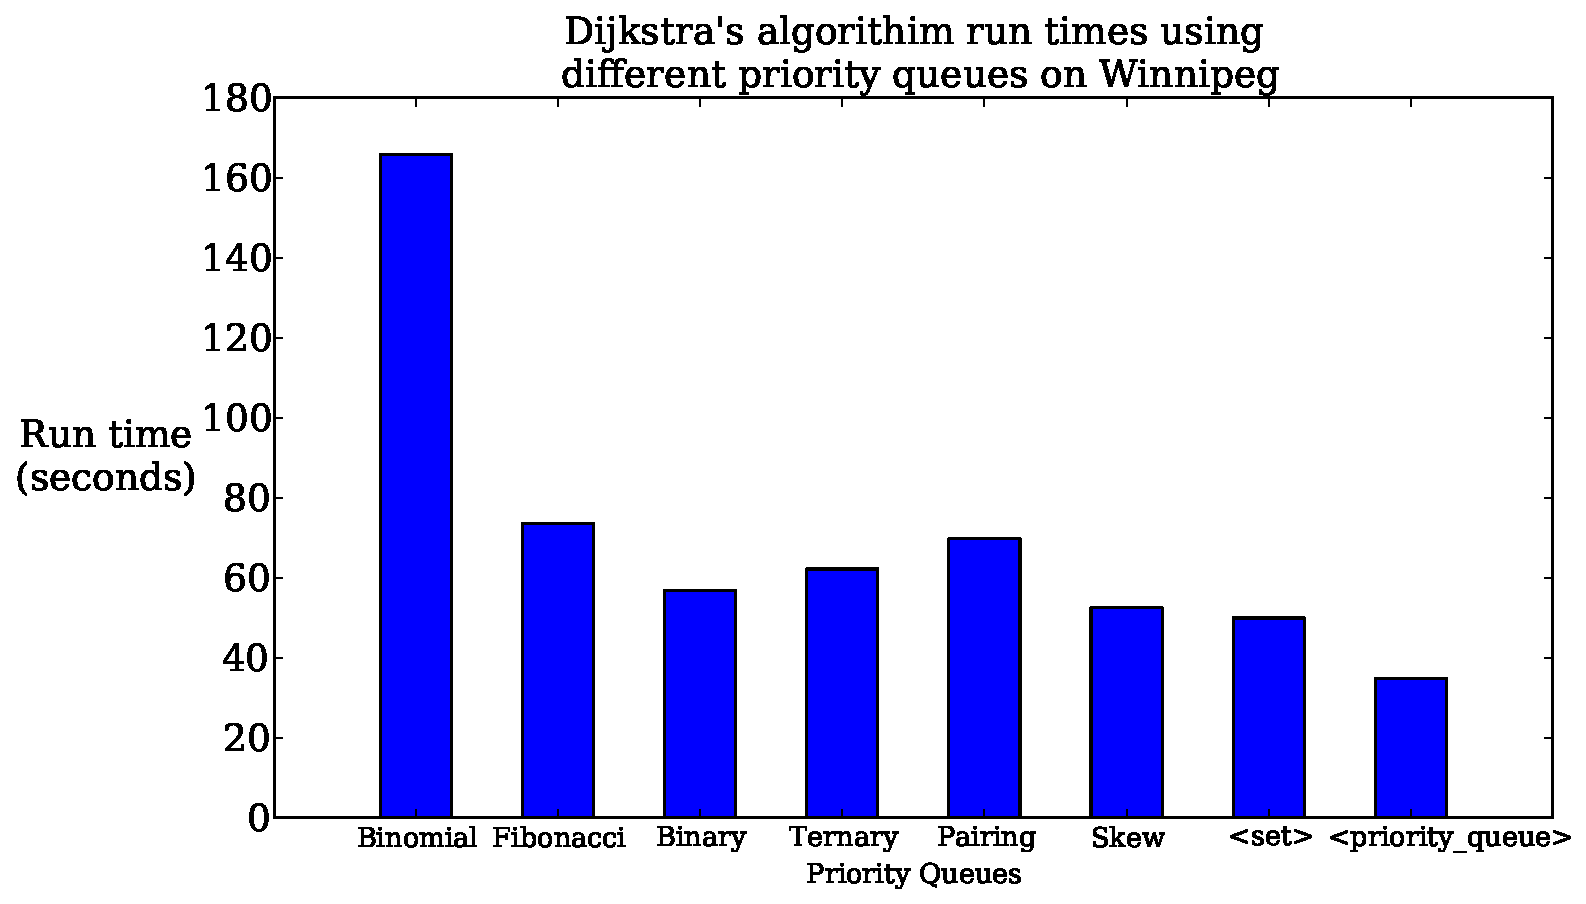
\includegraphics[page=1, width=\textwidth, height=.4\textheight]{img/pq_runtime}
    \caption{Full traffic assignment run times using Dijkstra's algorithm with different priority queues on Winnipeg, a total number of $547{,}344$ shortest paths are solved.}
    \label{fig:pq_runtime2}
\end{figure}
\begin{figure}[!ht]
    \centering
    \includegraphics[page=2, width=\textwidth, height=.4\textheight]{img/pq_runtime}
    \caption{Full traffic assignment run times using Dijkstra's algorithm with different priority queues on Chicago Sketch, a total number of $2{,}328{,}375$ shortest paths are solved.}
    \label{fig:pq_runtime}
\end{figure}

\subsection{Discussion on priority queues}
The priority queue implementation results show that
all of the heap implementations from the Boost library and $\langle$set$\rangle$ are worse than $\langle$priority\_queue$\rangle$.
The reason behind this can be explained using the Binary heap implementation.
It turns out that the implementation of $\langle$priority\_queue$\rangle$ is similar to Binary heap from the Boost library,
the only difference is their underlying storage of node information.
Nodes are stored using an array in the standard library version,
whereas the Boost library uses pointer references to keep track of 
the nodes.
Due to computer cache coherence,
it is known that accessing data from a nearby random access memory (RAM) locations in a short period of time is faster than accessing from distant memory locations.
This is due to cache memory access being much faster than RAM access,
and internally a block of memory is pre-fetched into the cache in the hope they will be accessed in a short period of time.
In the shortest path algorithms,
the heap tree needs to be searched over and over again in a short period of time when nodes are being scanned and inserted.
The standard library version uses an array where data are stored linearly in a nearby location,
so it is much faster than the pointer based version where memory is allocated in random locations when nodes are inserted.

\subsection{Discussion of Fibonacci heap}
Here we discuss the reason behind Fibonacci heap not performing well despite its $O(1)$ amortized time Decrease-Key operation.
As described in the two priority queue sections (Section~\ref{sec:pq} and \ref{sec:pq_implementation}),
the Decrease-Key operation is used to change the distance label of a node when the node is already in the heap.
It was discovered that the $O(1)$ time has a very high constant factor,
and Fibonacci heap only works well if the underlying graph is large and dense (i.e.\ every node connects to almost every other node).
This discovery comes from the fact that 
the Decrease-Key operation is only used frequently when the graph is dense,
so cumulatively its high constant $O(1)$ time will perform better compared to $O(\log(N))$ time in other heap implementations, where $N$ need to be a large number.

We confirm our graph is indeed not dense and the Decrease-Key is not used frequent.
We find that all of our graphs are very sparse.
The degree of any node of any graph is no more than 5,
as it is already really rare to have an intersection with 5 roads connected.
The graphs only have about 0.4\% to 0.6\% of arcs in the corresponding complete graph (every node connects to every other node).
We also find that in all of the experimented graphs when using Dijkstra's algorithm,
the probability of using Decrease-Key on any node is only around 1 to 5 percent.

\section{Results on shortest path algorithms} \label{sec:allresults}
In Section~\ref{sec:pq_results} we have identified  $\langle$priority\_queue$\rangle$ to be the most suitable (efficient) data structure to be used in Dijkstra's algorithm.
We use $\langle$priority\_queue$\rangle$, implement and test the following algorithms:
\begin{itemize}
        \item Bellman-Ford-Moore algorithm (existing),
        \item Dijkstra's algorithm,
        \item Bidirectional Dijkstra's algorithm,
        \item A* search,
        \item Bidirectional A* search.
\end{itemize}
%Therefore we use $\langle$priority\_queue$\rangle$ from the C++ standard template library and implement Dijkstra's algorithms and A* search, as well as their bidirectional versions.
Figure~\ref{fig:allresults} shows the performance of the mentioned algorithms on the Anaheim, Barcelona, Winnipeg and Chicago Sketch networks
(see Table~\ref{table:allresults} of Appendix~\ref{appendix} for exact numerical results).
The networks are spaced out on the horizontal axis to show their relative sizes, i.e.\ the number of O-D pairs.

Bellman-Ford-Moore algorithm has the worst performance while A* search has the best performance on all networks.
The bidirectional versions of Dijkstra's algorithm and A* search are more than twice slower than their unidirectional versions.

\begin{figure}[!ht]
    \centering
    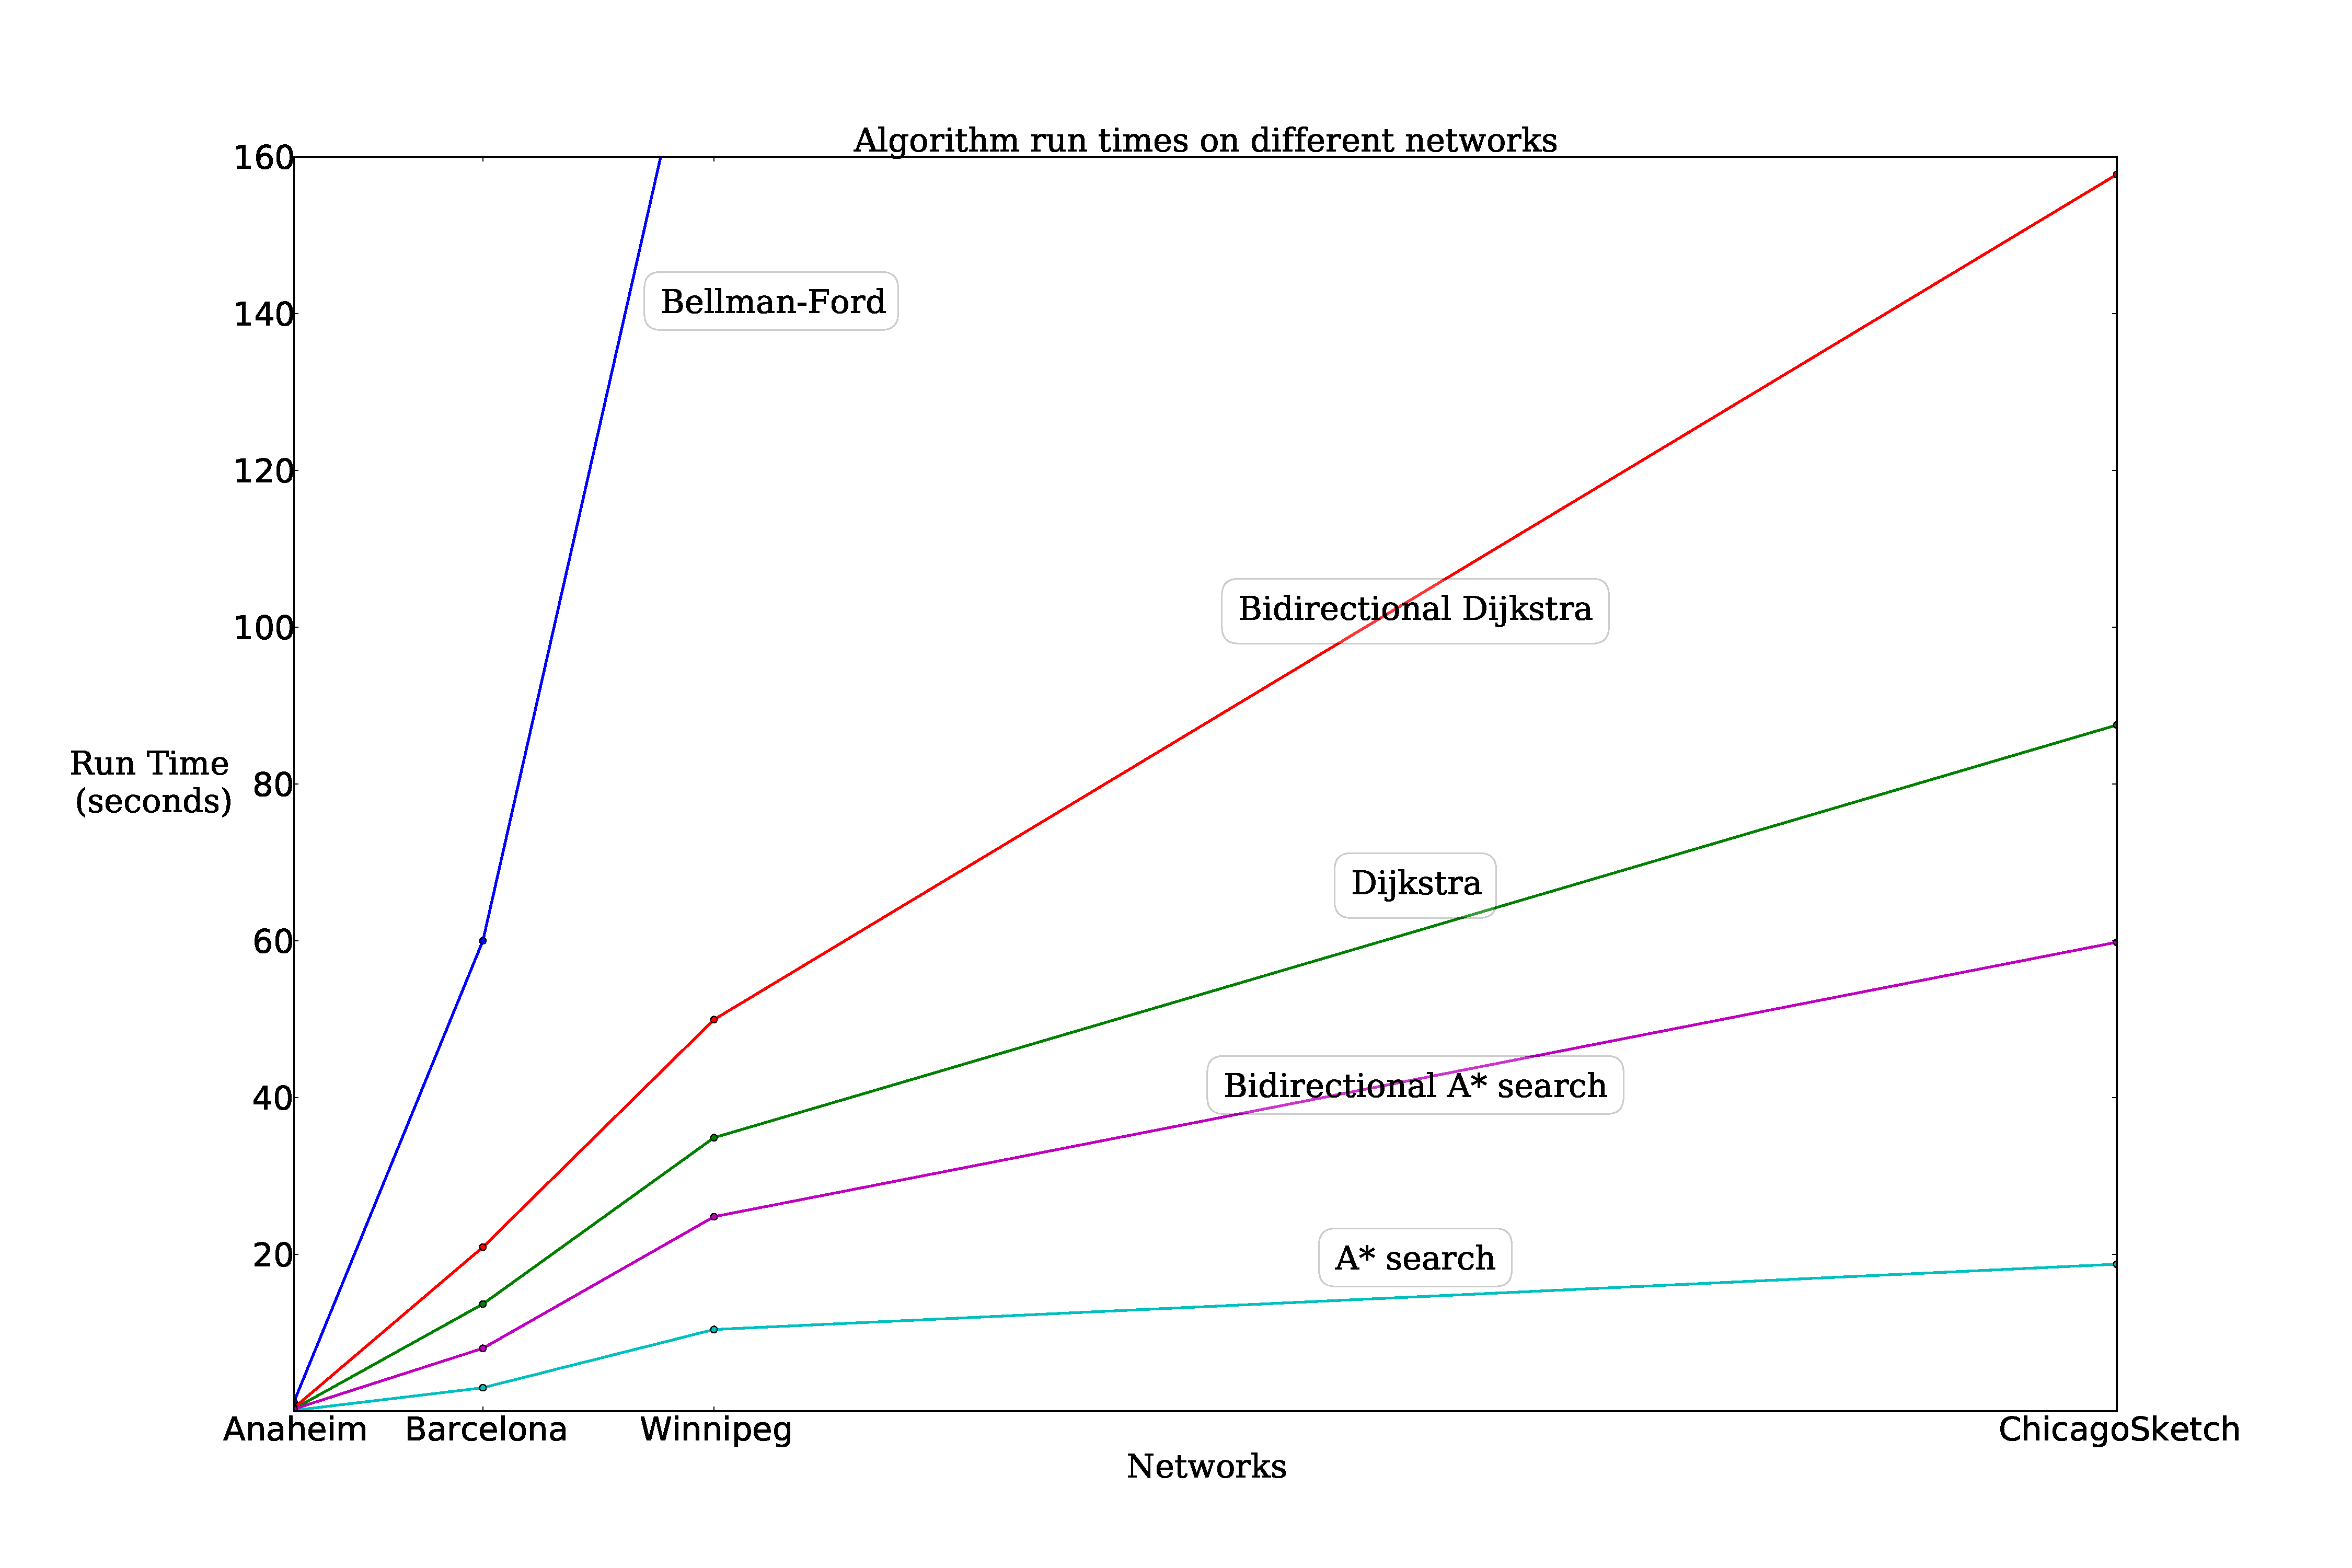
\includegraphics[width=\textwidth]{img/runtime}
    \caption{Run time performances of different algorithms on different networks}
    \label{fig:allresults}
\end{figure}

\subsection{Discussion of shortest path algorithms}
In this section we investigate the reason for the worse performances of the bidirectional algorithms compared to their unidirectional versions. 

First we examine whether search areas of the algorithms are what is expected.
Figure~\ref{fig:long_sptree} shows the shortest path trees of the point-to-point algorithms, 
where the origin and destination nodes are placed on opposite sides of Chicago Sketch network.
It can be seen that Dijkstra's algorithm scans the entire network.
Bidirectional Dijkstra scans almost the entire network with some nodes left out on the sides of the network.
Bidirectional A* scans a slightly larger region near the origin and destination nodes,
and the A* search scans just a few nodes along the shortest path.
The behaviour of the algorithms are shown further in Figure~\ref{fig:short_sptree},
where the origin and destination are placed close to each other.
It can be seen that both Dijkstra's algorithm and its bidirectional version scan almost half of the graph,
where the bidirectional version scans fewer nodes.
A* search and its bidirectional search scan a small portion of the graph,
and they do not scan the area behind the origin and destination node compared to the Dijkstra's algorithm.

The search areas of the bidirectional Dijkstra's algorithms match what is expected,
but not the run times when compared to the unidirectional version.
The reason for reduction in run time is due to our implementations.
In both forward and backward search,
the current shortest path $\mu$ needs to be updated every time a node is scanned,
and the stopping criterion needs to be checked when a node is labelled.
Furthermore,
once the algorithm terminates,
we need to retrieve the shortest path in both directions by following node predecessors and concatenate them together for the full shortest path.
So it is concluded that these additional computations slowed down the run times.

For A* search,
the bidirectional version always scans more nodes than the unidirectional version.
This is due to the worse bounds of heuristic estimates calculated in the bidirectional search compared to the unidirectional version,
That is, heuristic estimates need to be averaged from the forward and backward search in order to find the correct shortest path.
Since the bidirectional version has similar stopping criterion compared to the bidirectional Dijkstra's algorithm,
it is easy to understand why bidirectional A* has a worse performance.

Finally, there is one thing that needs to be pointed out for A* search.
A* search requires to run Dijkstra's algorithm on all nodes (not zones) in the network to obtain the heuristic estimates (zero-flow travel times from every node to every destination) and store the travel time values (not the paths).
This procedure is similar to that of pre-processing algorithms,
where we need to pre-process the network so subsequent queries can be made faster.
In our A* search results, the run times included the pre-processing and the overall run time is still faster than all the other tested algorithms.

\begin{figure}
    \centering
    \begin{subfigure}{.5\textwidth}
        \centering
        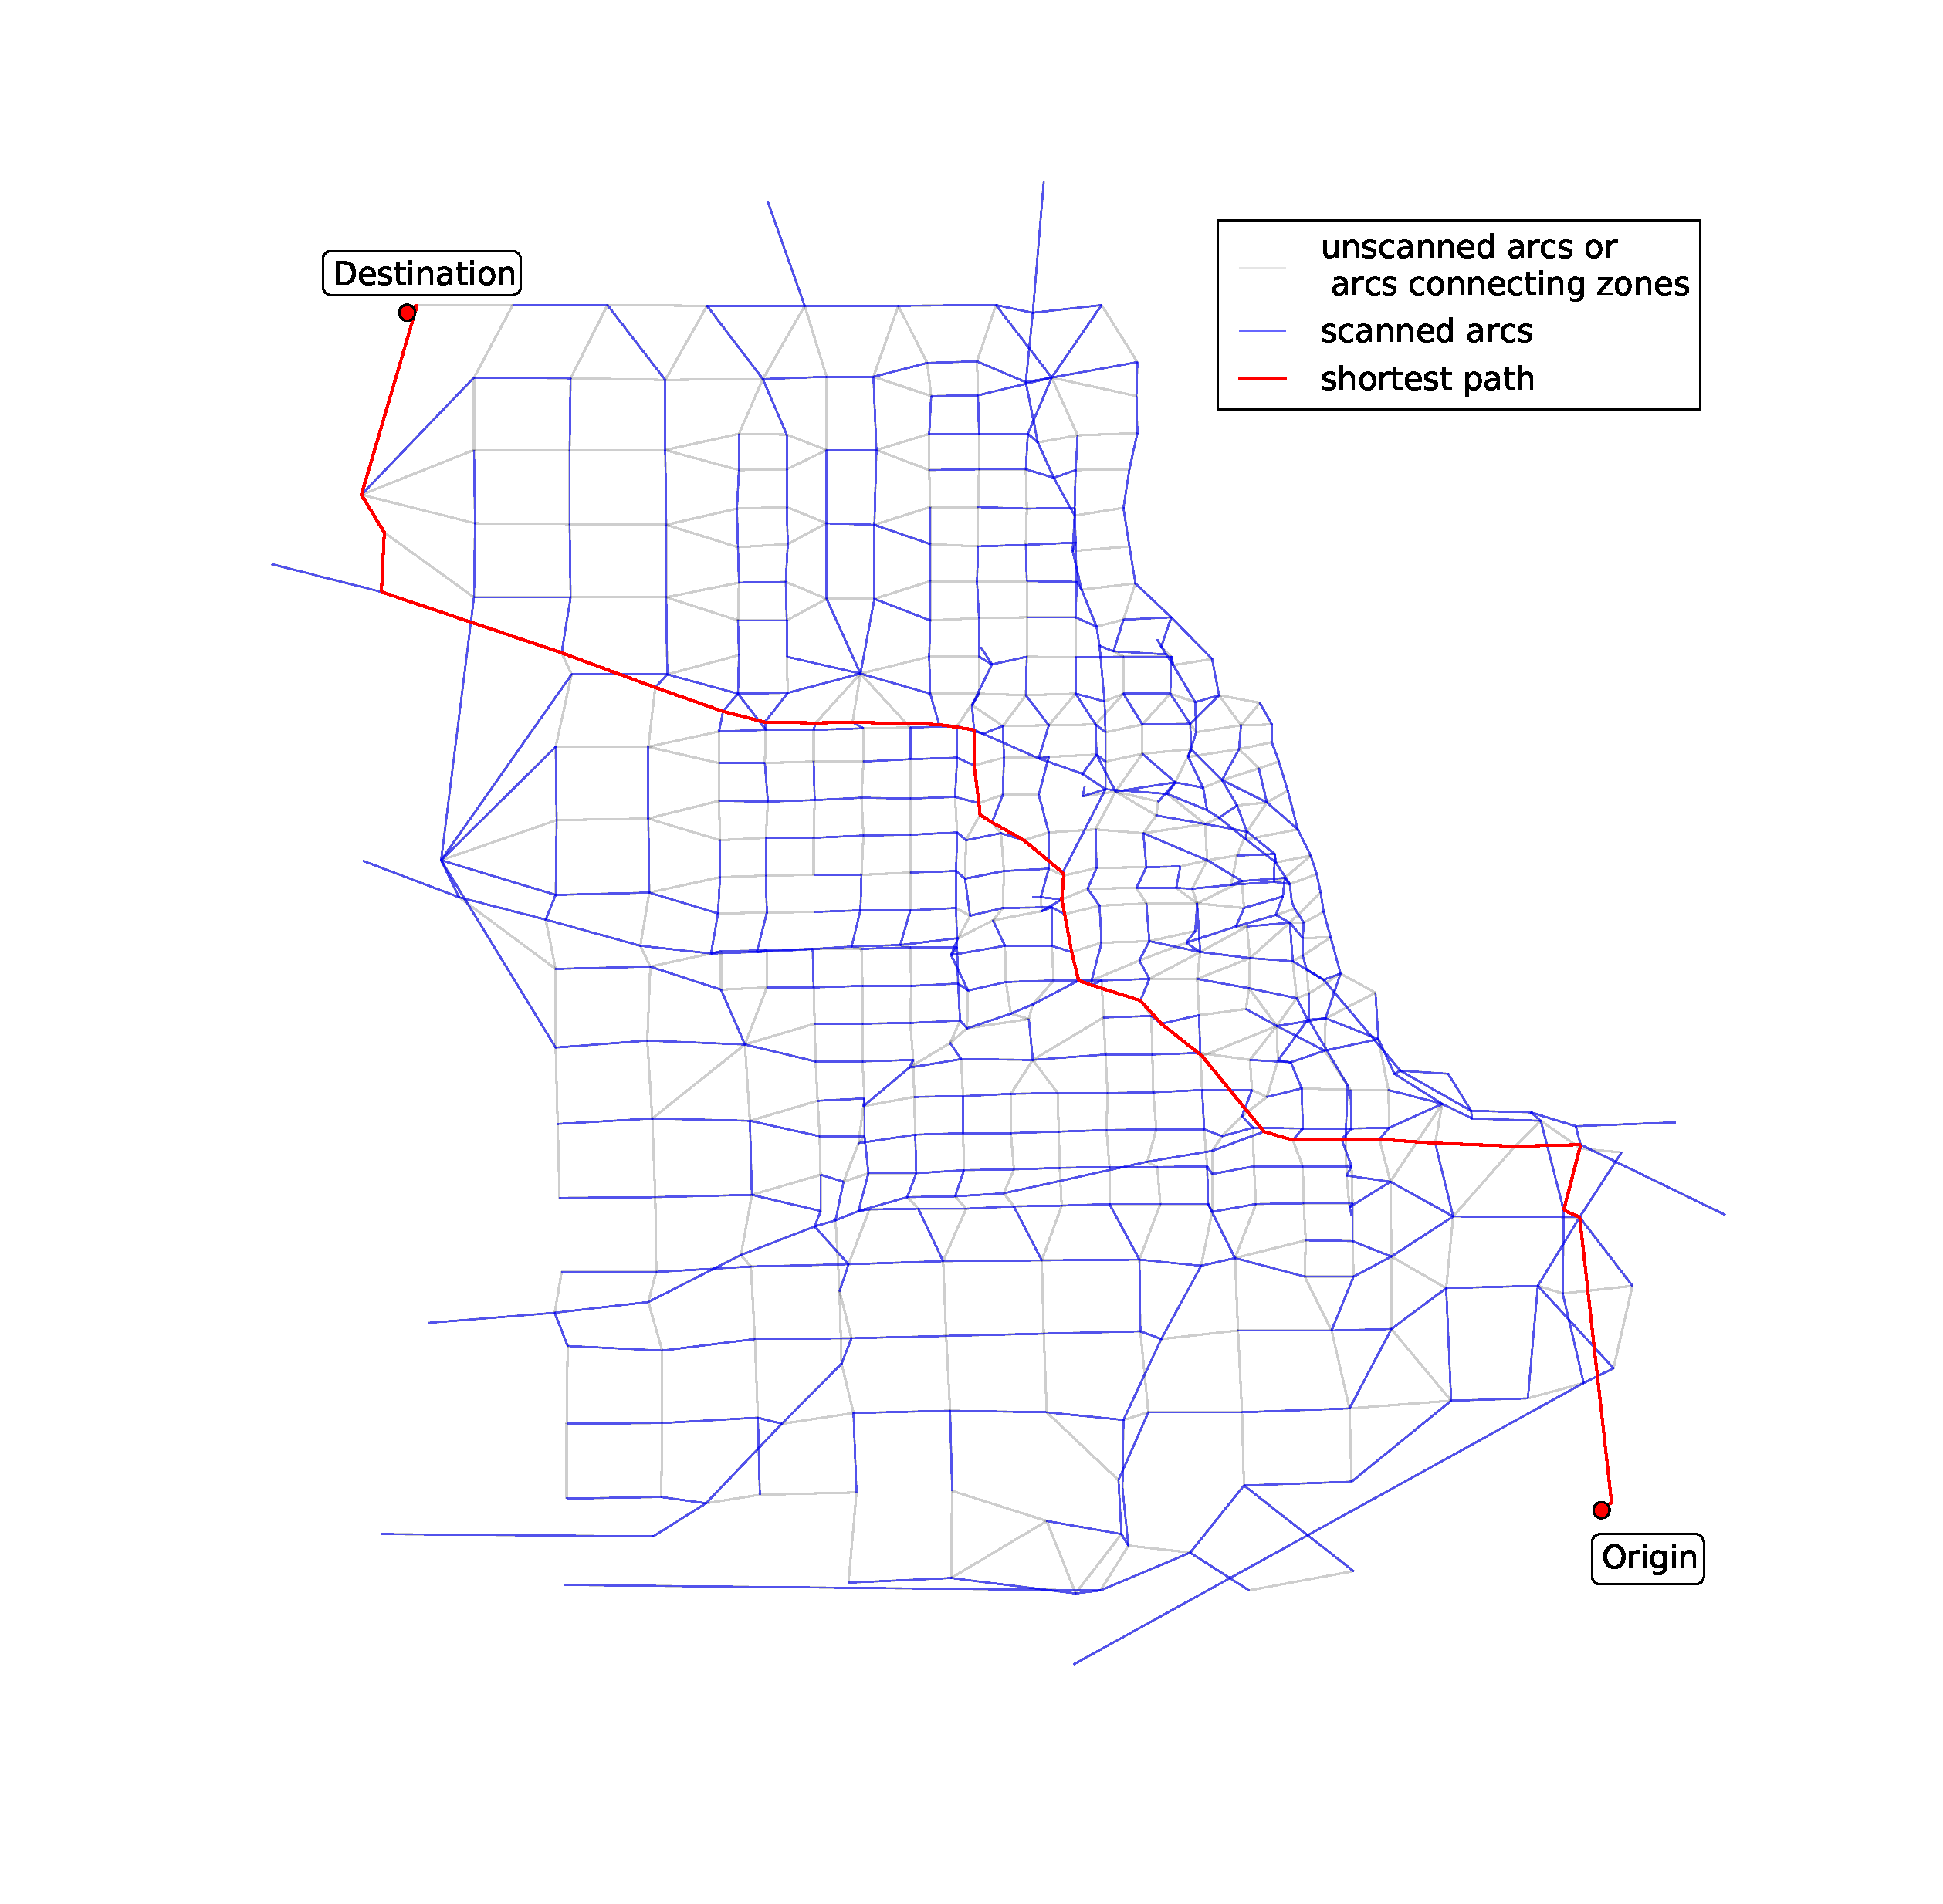
\includegraphics[width=\textwidth,trim=120px 120px 48px 120px,clip]{img/chicago_dijkstra}
        \caption{Dijkstra}
        \label{fig:chicago_dijkstra}
    \end{subfigure}%
    \begin{subfigure}{.5\textwidth}
        \centering
        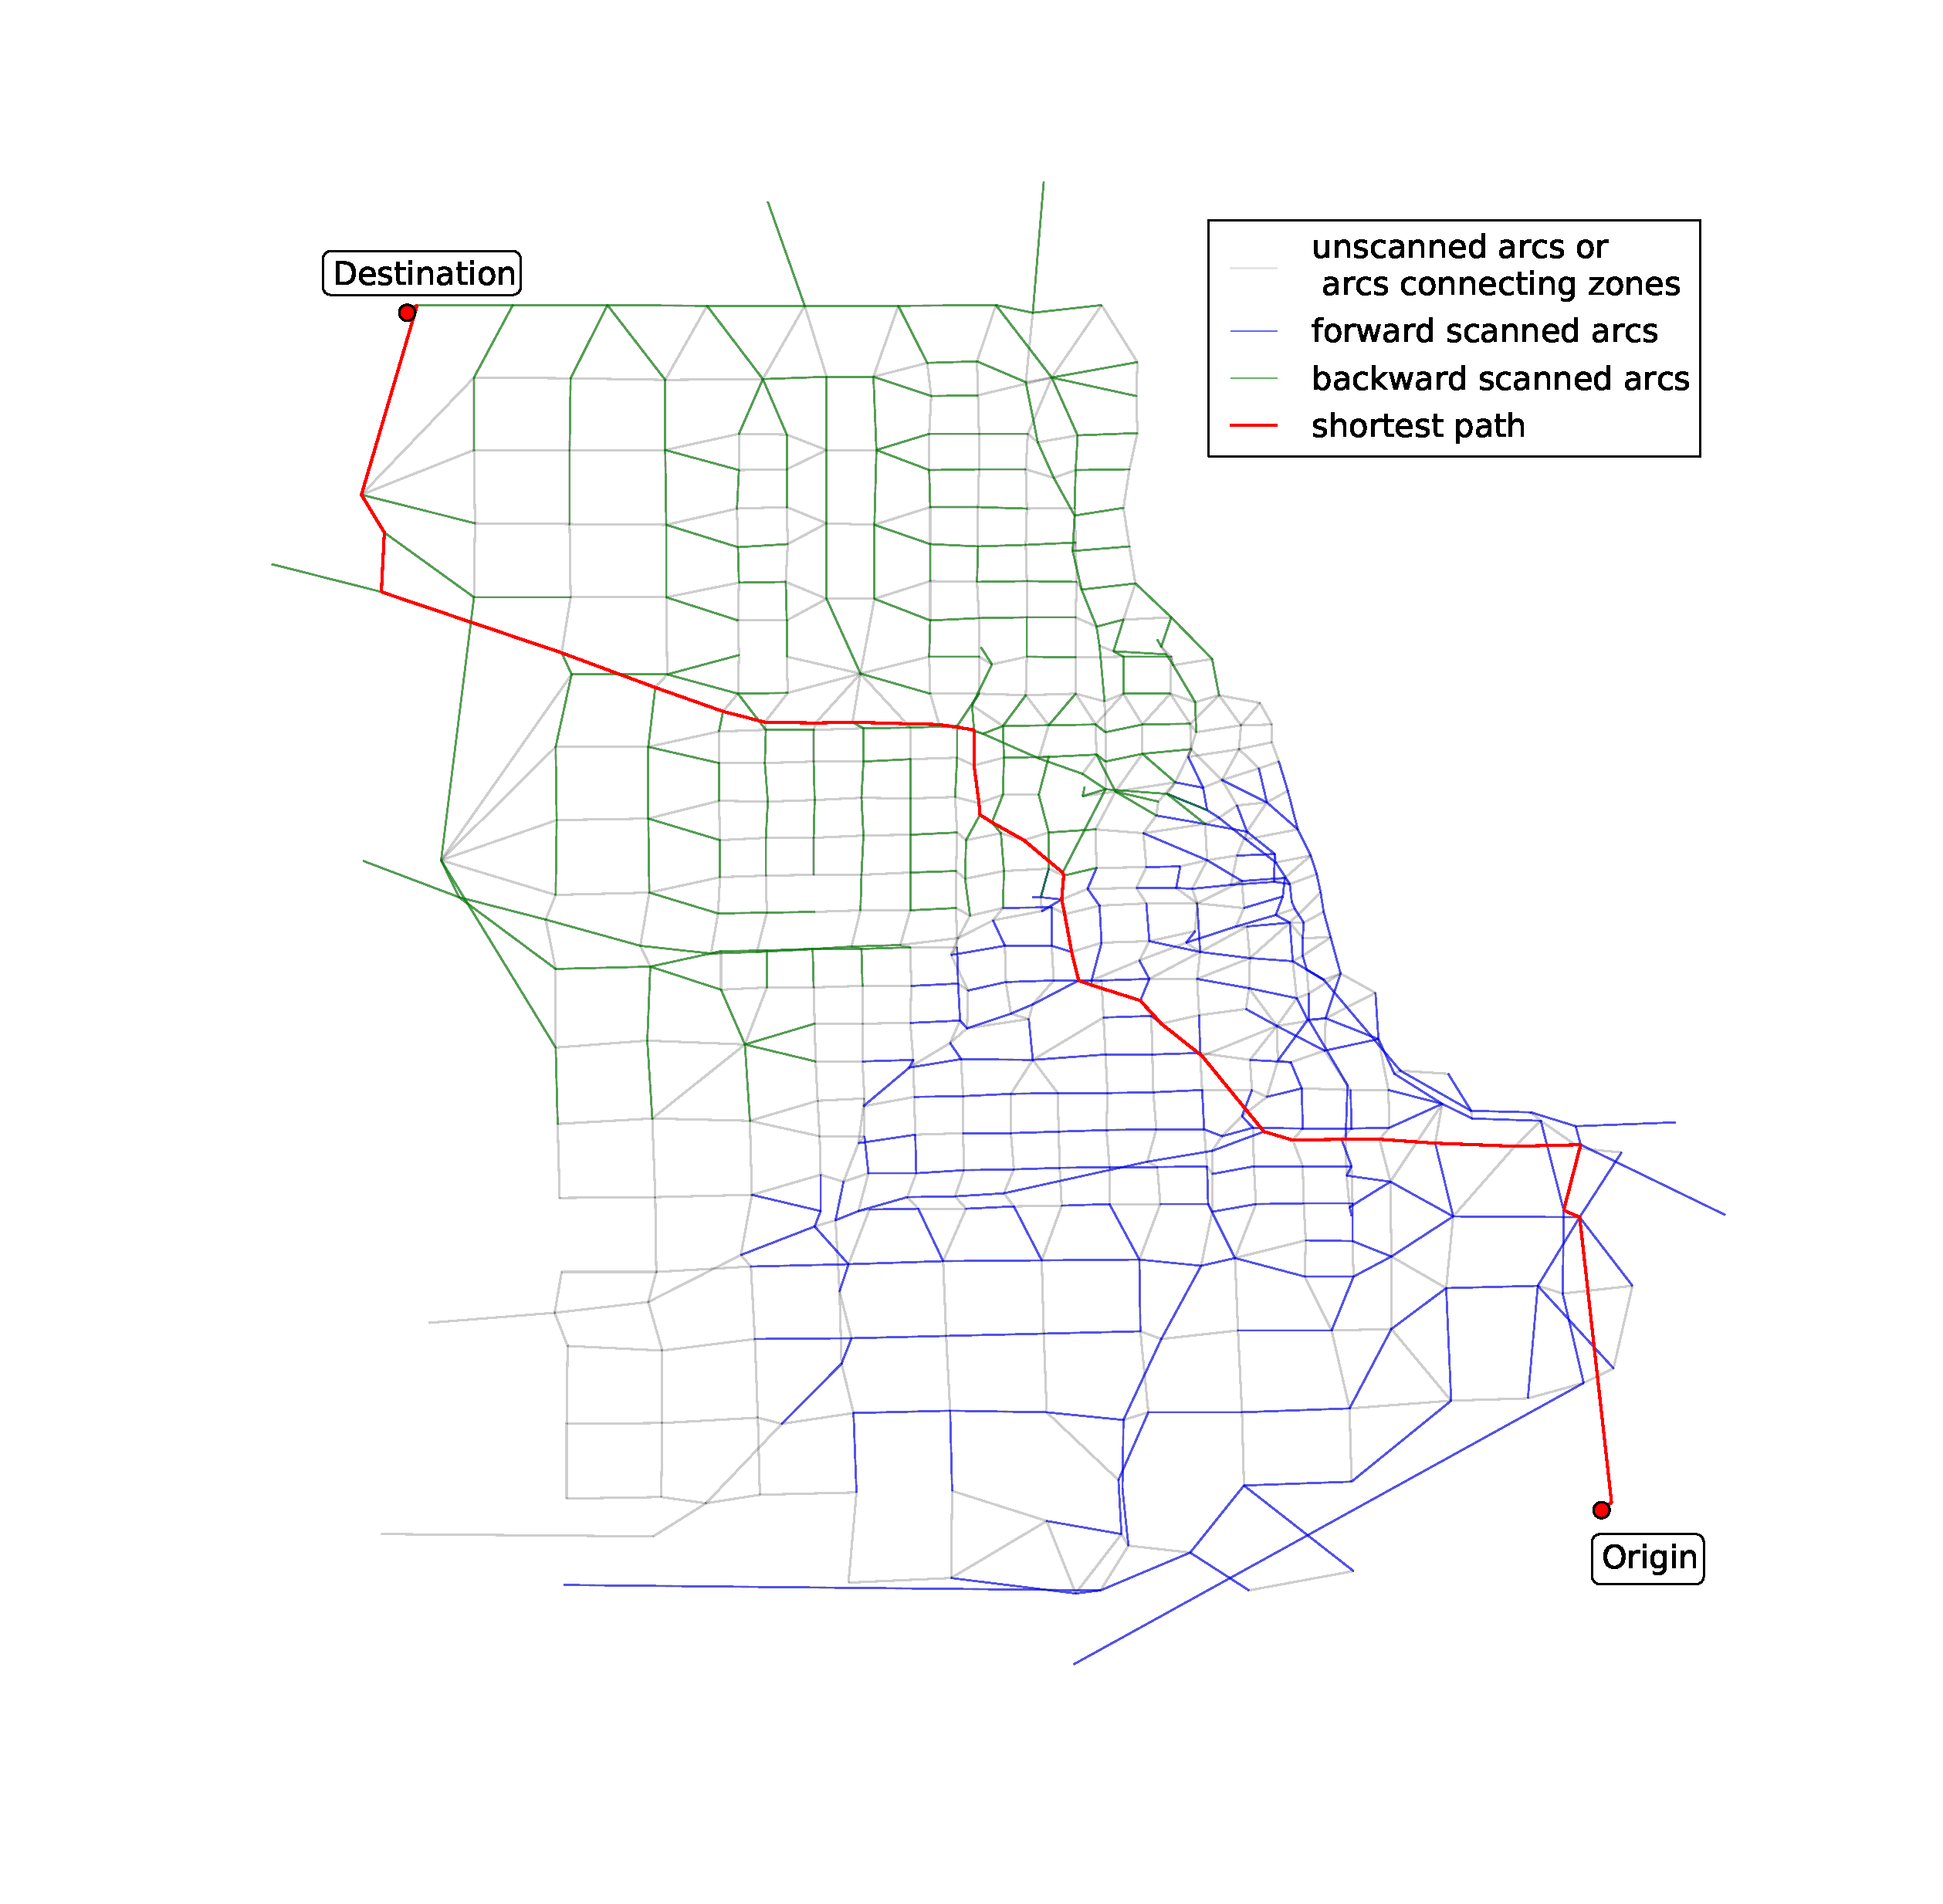
\includegraphics[width=\textwidth,trim=120px 120px 48px 120px,clip]{img/chicago_bidirect}
        \caption{Bidirectional Dijkstra}
        \label{fig:chicago_bidirect}
    \end{subfigure}
    \begin{subfigure}{.5\textwidth}
        \centering
        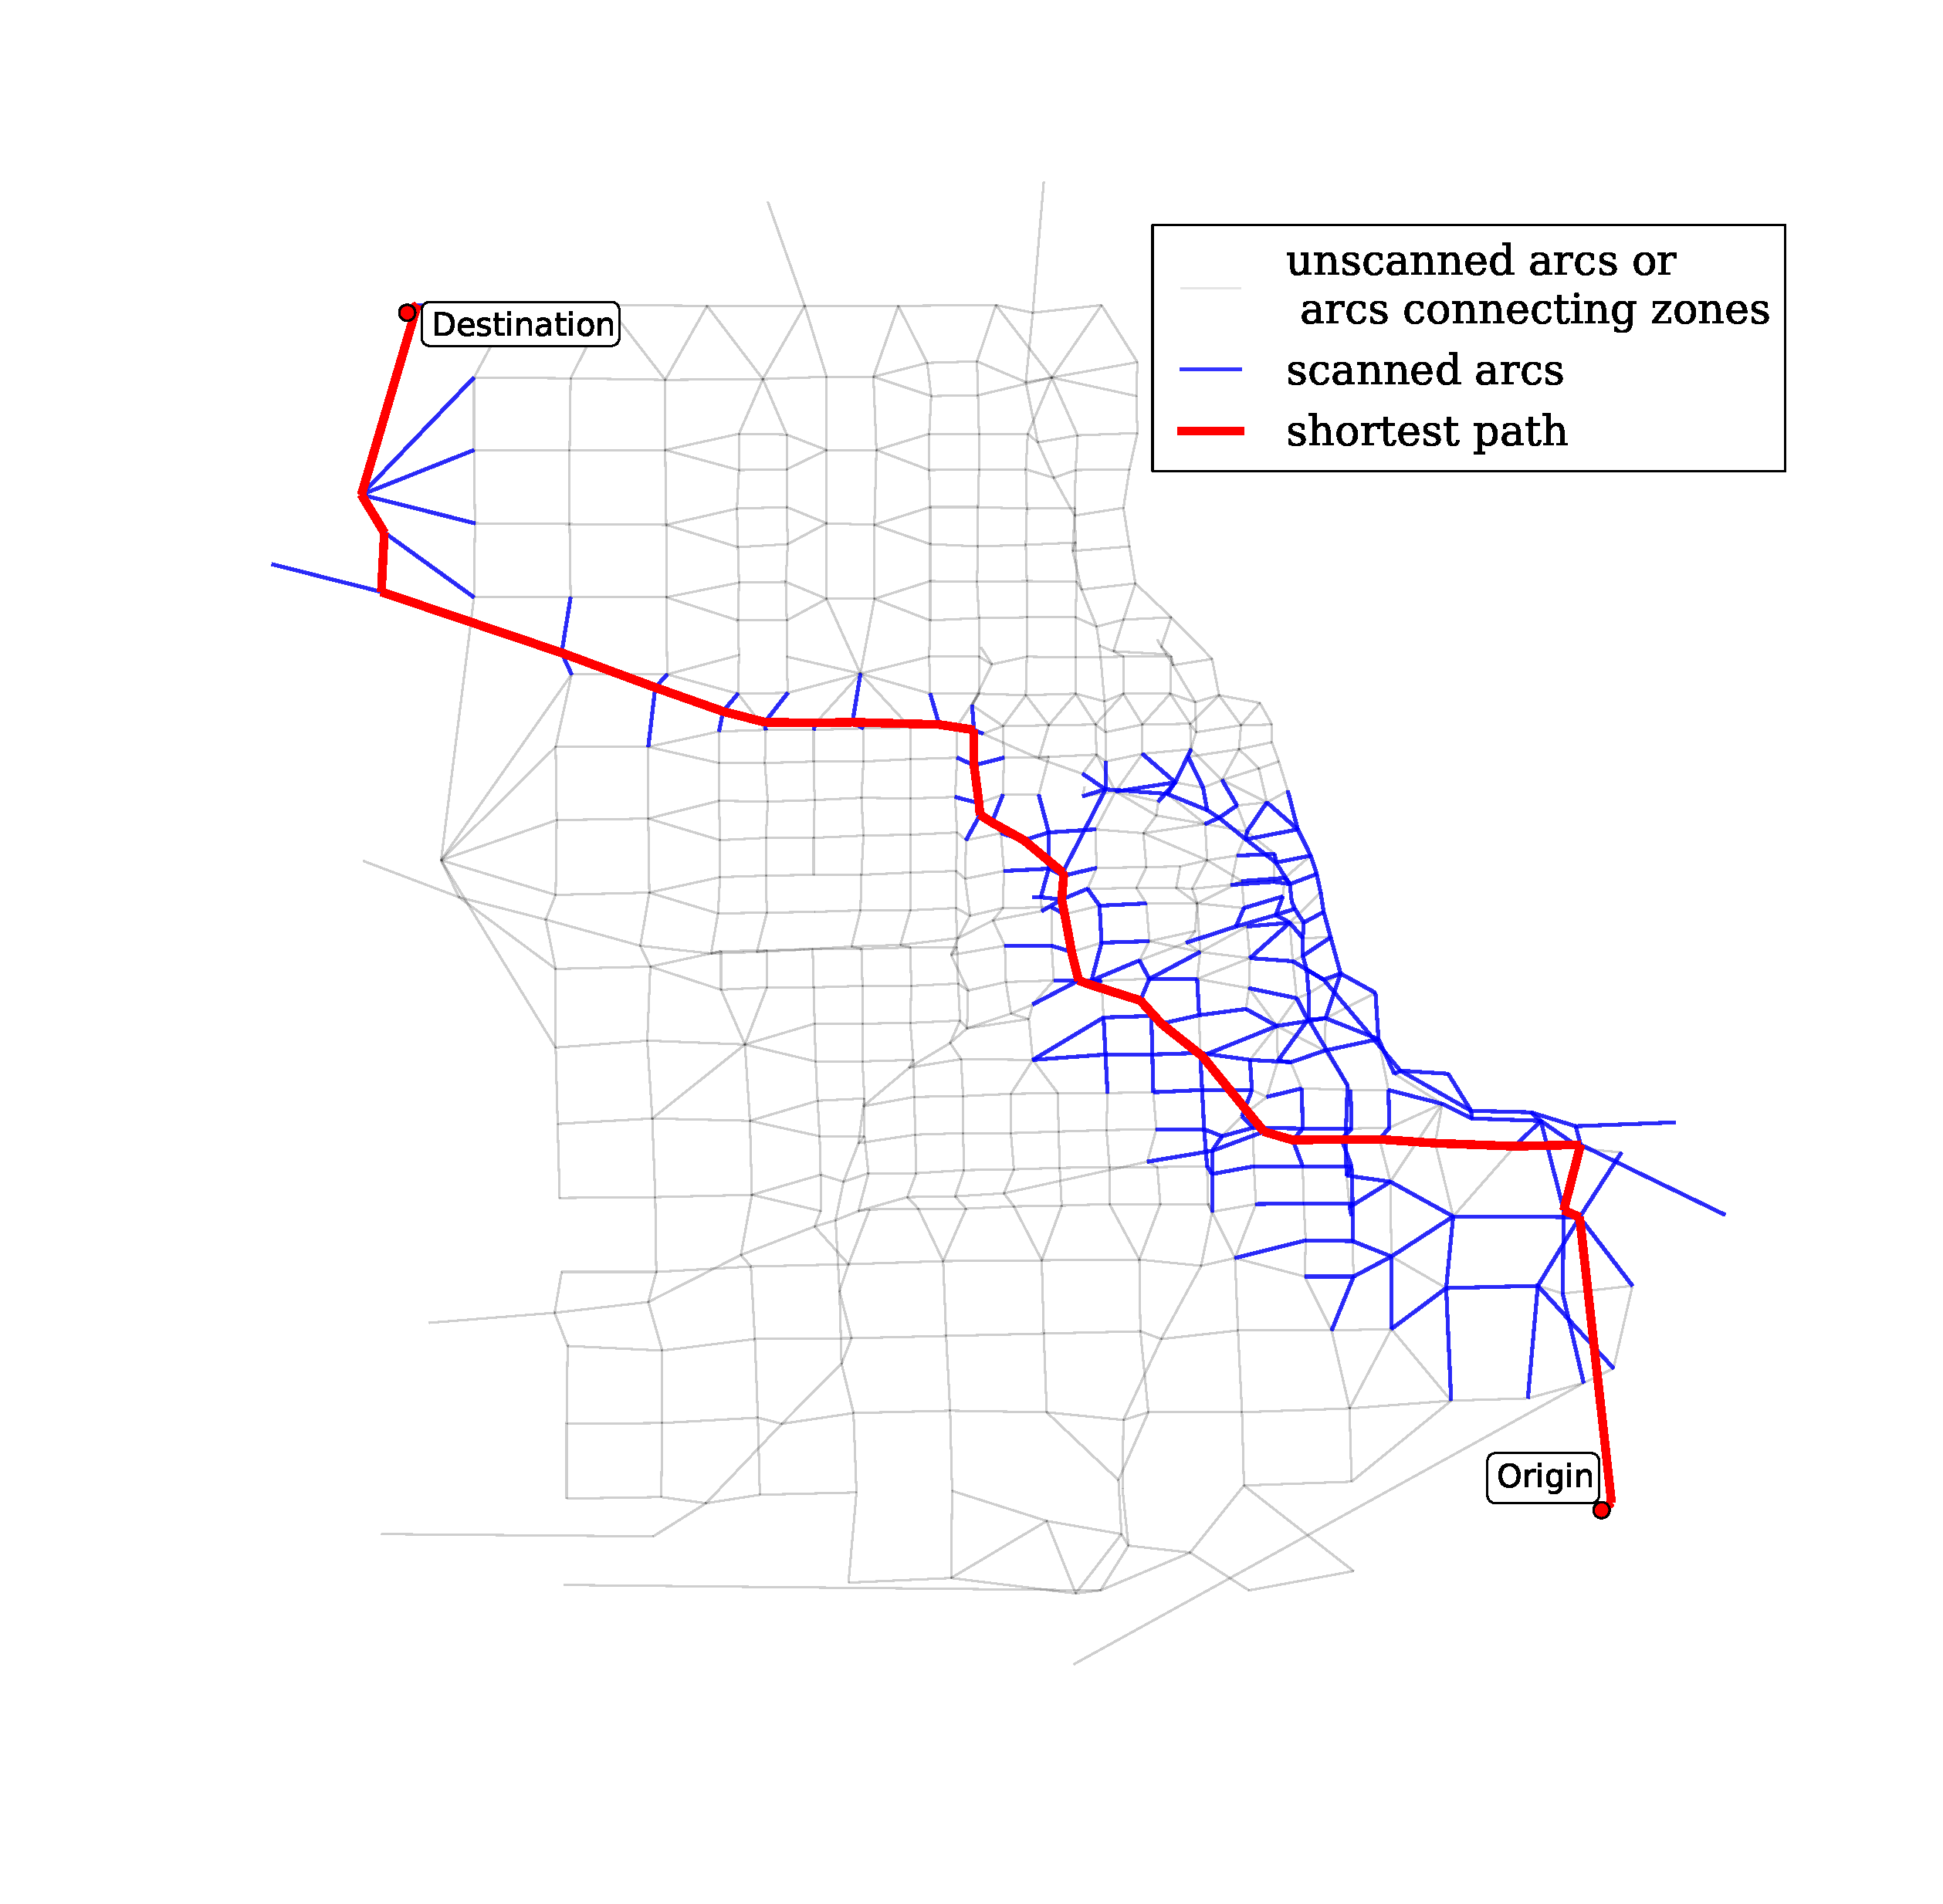
\includegraphics[width=\textwidth,trim=120px 120px 48px 0px,clip]{img/chicago_astar}
        \caption{A* Search}
        \label{fig:chicago_astar}
    \end{subfigure}%
    \begin{subfigure}{.5\textwidth}
        \centering
        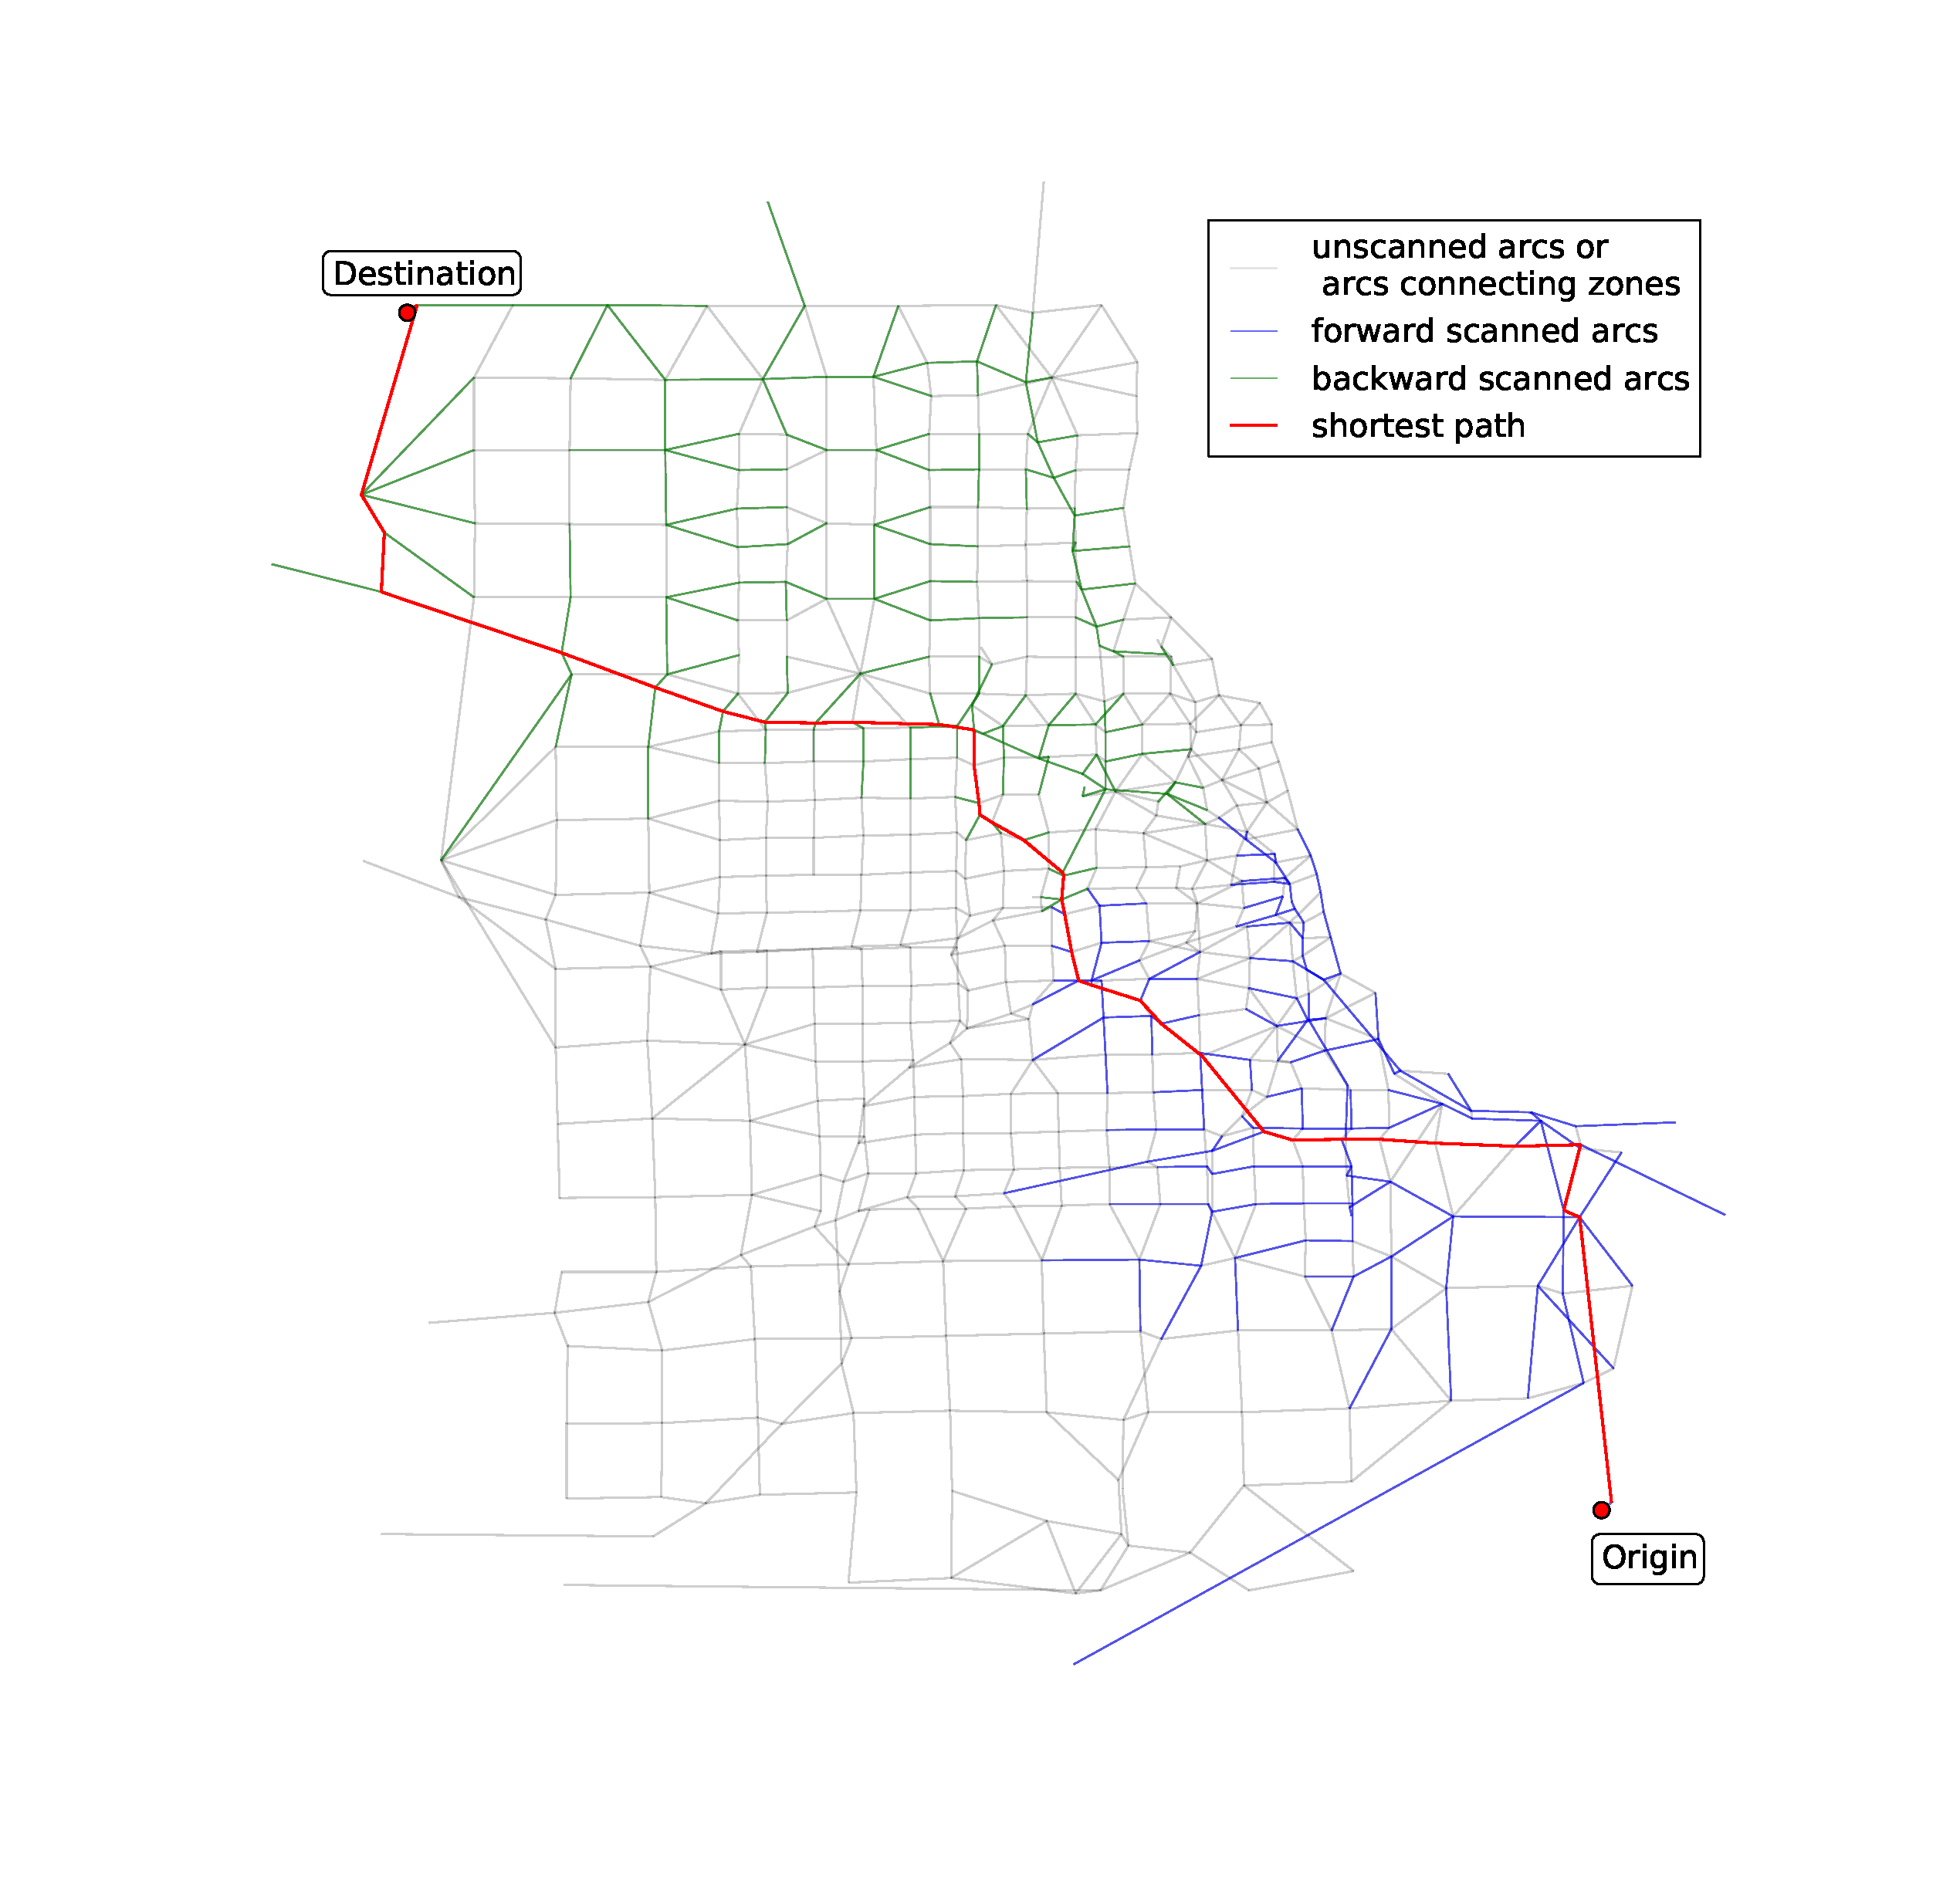
\includegraphics[width=\textwidth,trim=120px 120px 48px 0px,clip]{img/chicago_astar_bidirect}
        \caption{Bidirectional A* Search}
        \label{fig:chicago_astar_bidirect}
    \end{subfigure}
    \vspace{1em}
    \caption{Shortest path tree between two distant nodes in the Chicago Sketch network}
    \label{fig:long_sptree}
\end{figure}

\begin{figure}
    \centering
    \begin{subfigure}{.5\textwidth}
        \centering
        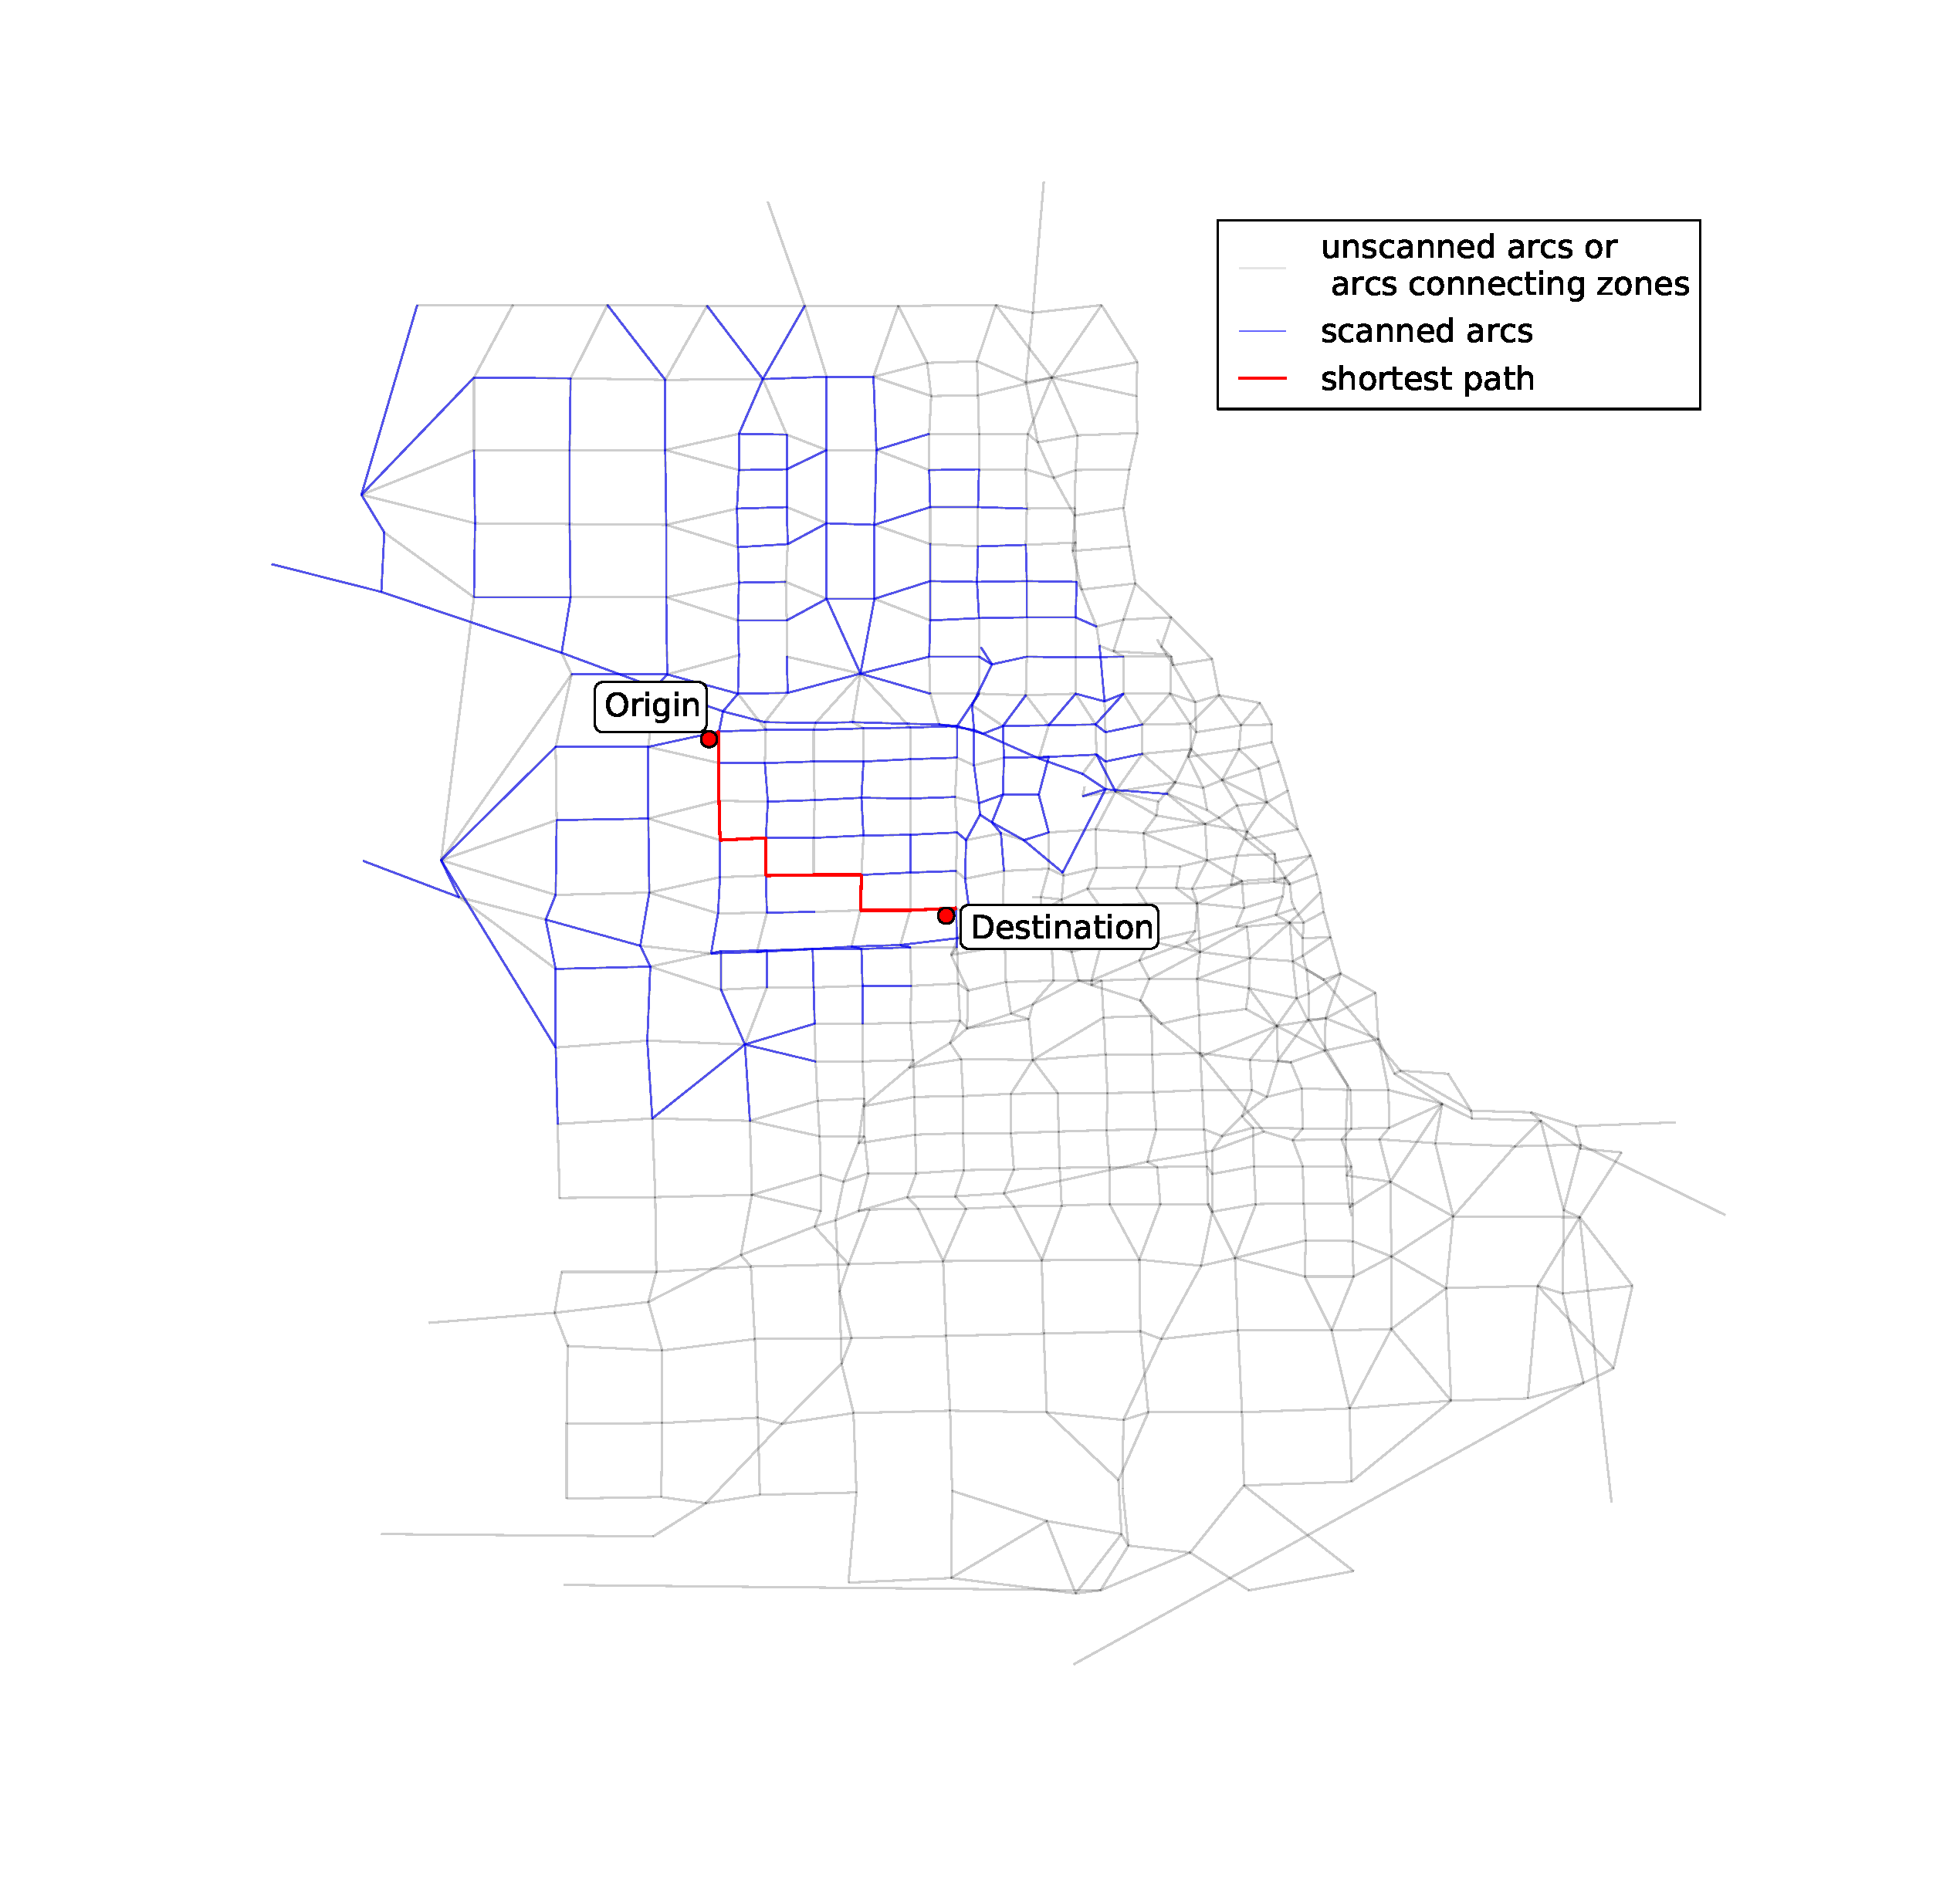
\includegraphics[width=\textwidth,trim=120px 120px 48px 120px,clip]{img/chicago_dijkstra2}
        \caption{Dijkstra}
        \label{fig:chicago_dijkstra2}
    \end{subfigure}%
    \begin{subfigure}{.5\textwidth}
        \centering
        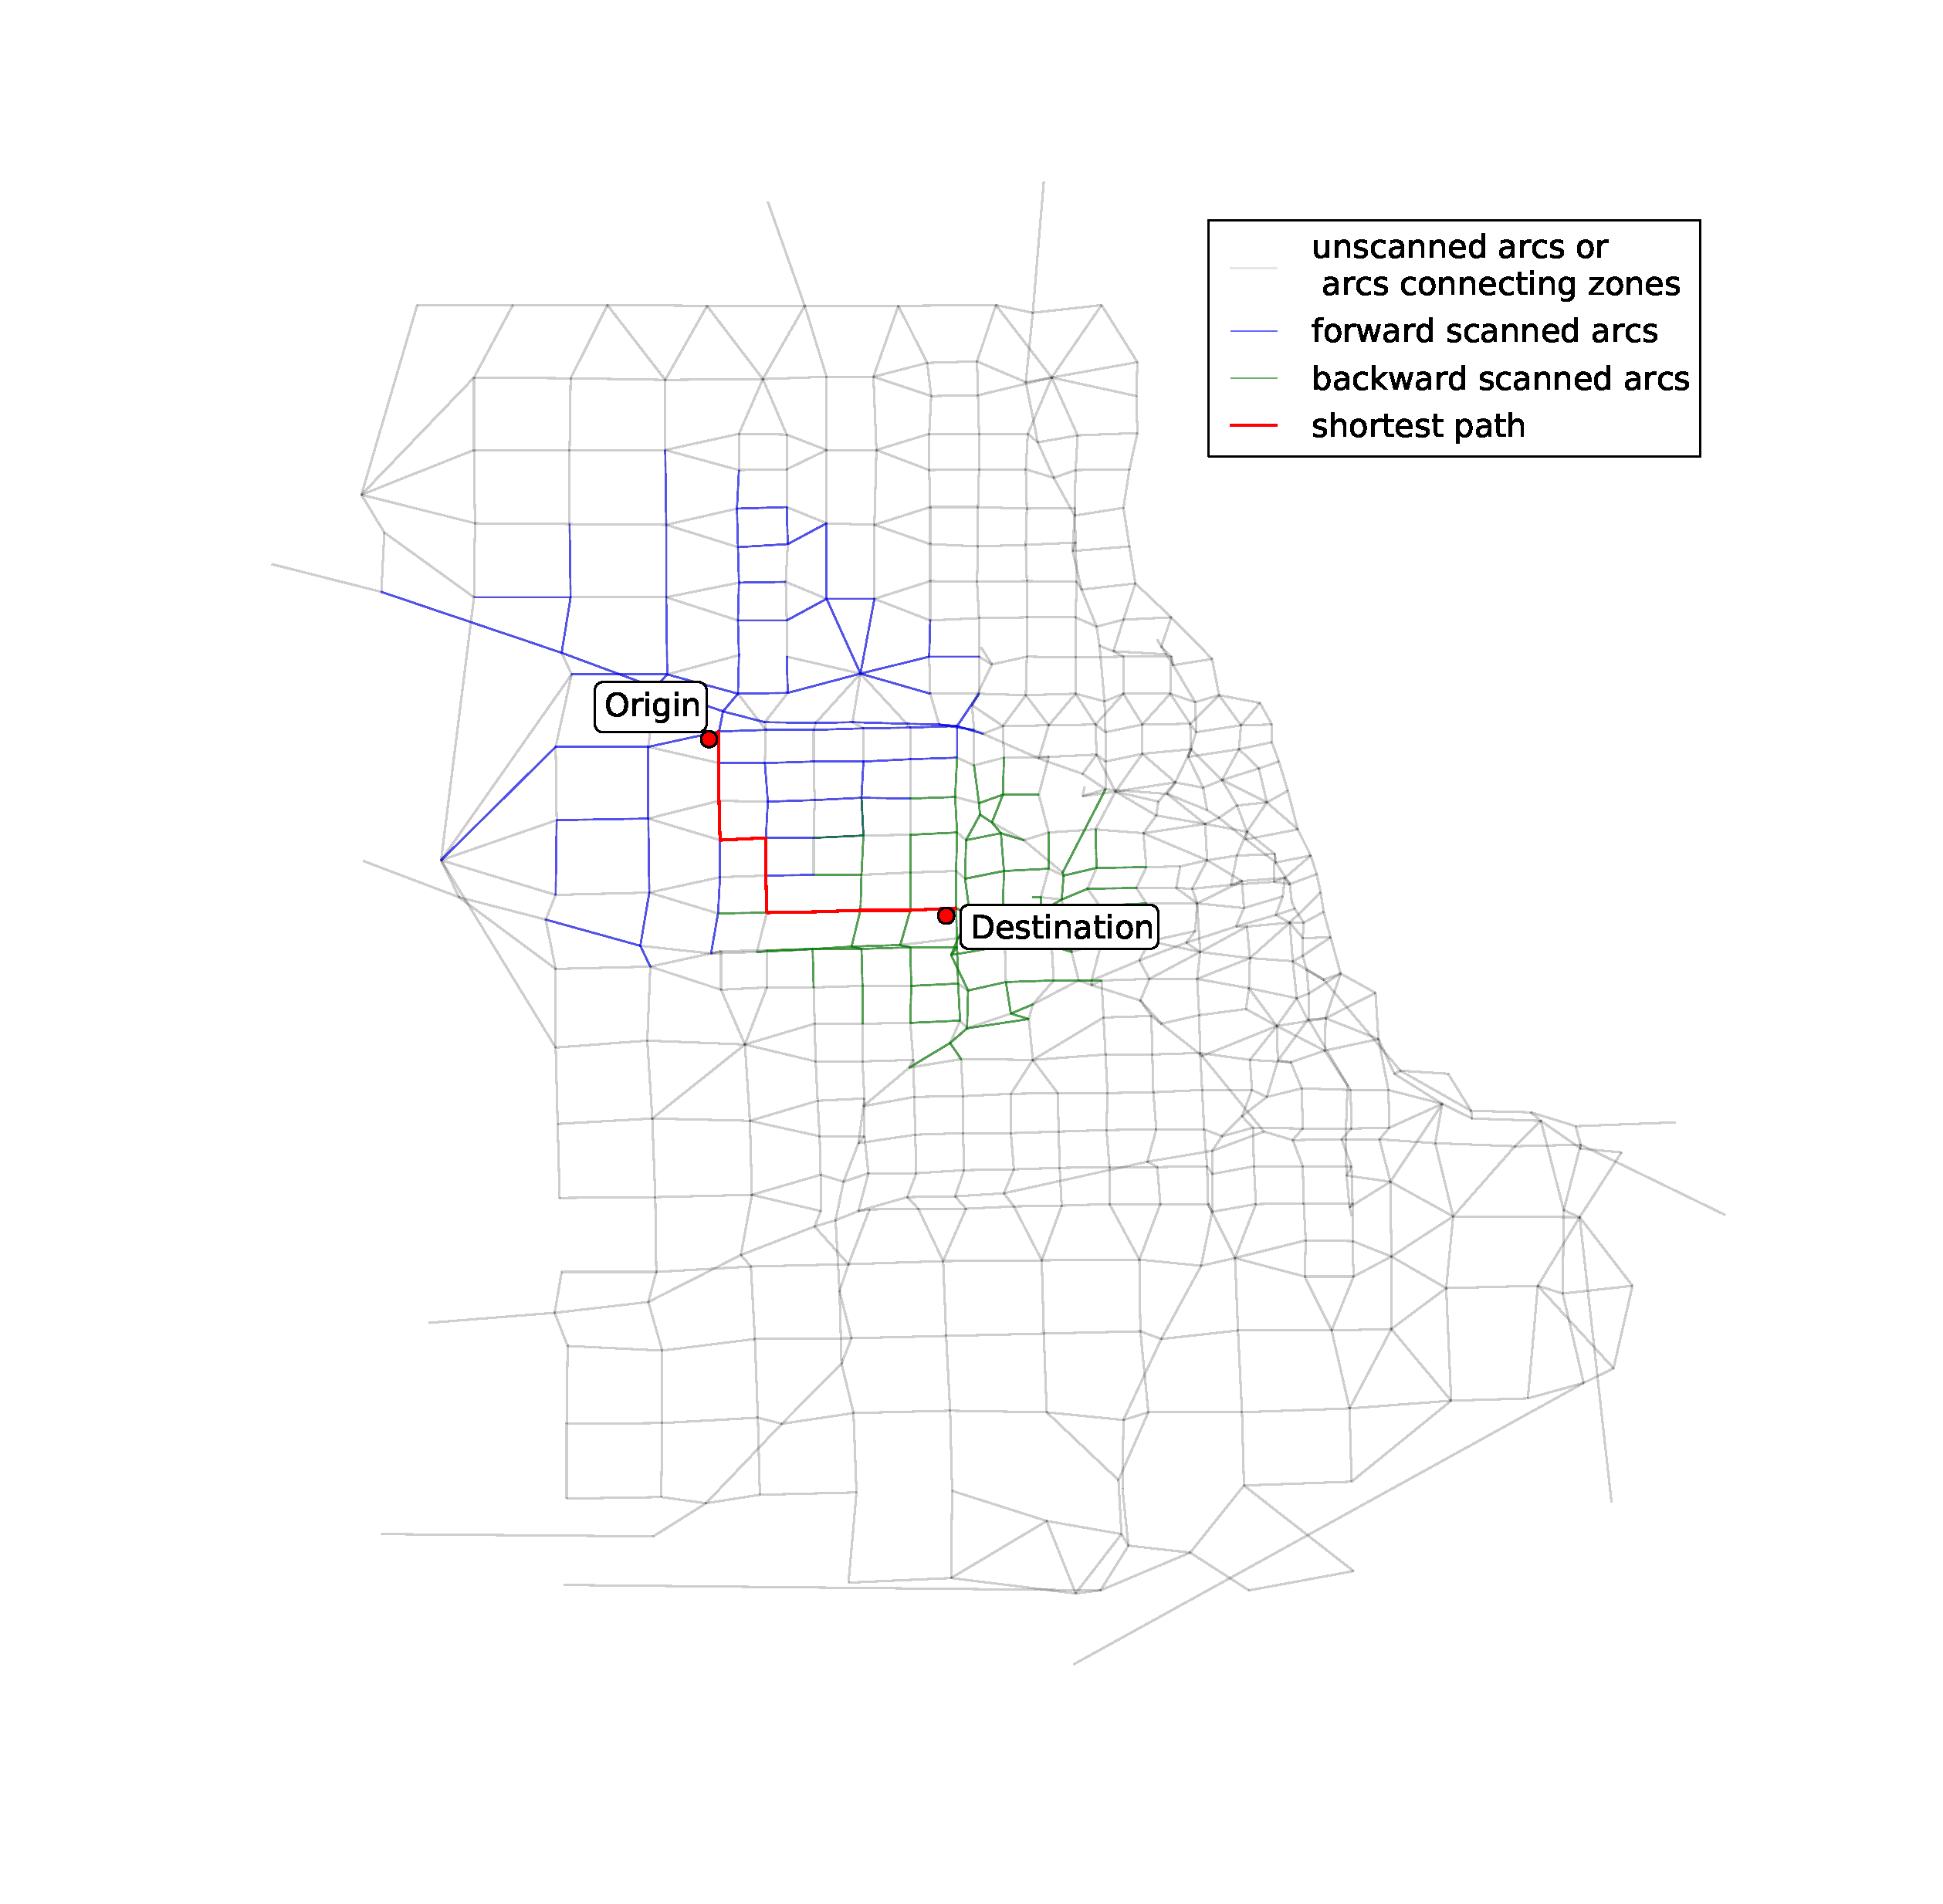
\includegraphics[width=\textwidth,trim=120px 120px 48px 120px,clip]{img/chicago_bidirect2}
        \caption{Bidirectional Dijkstra}
        \label{fig:chicago_bidirect2}
    \end{subfigure}
    \begin{subfigure}{.5\textwidth}
        \centering
        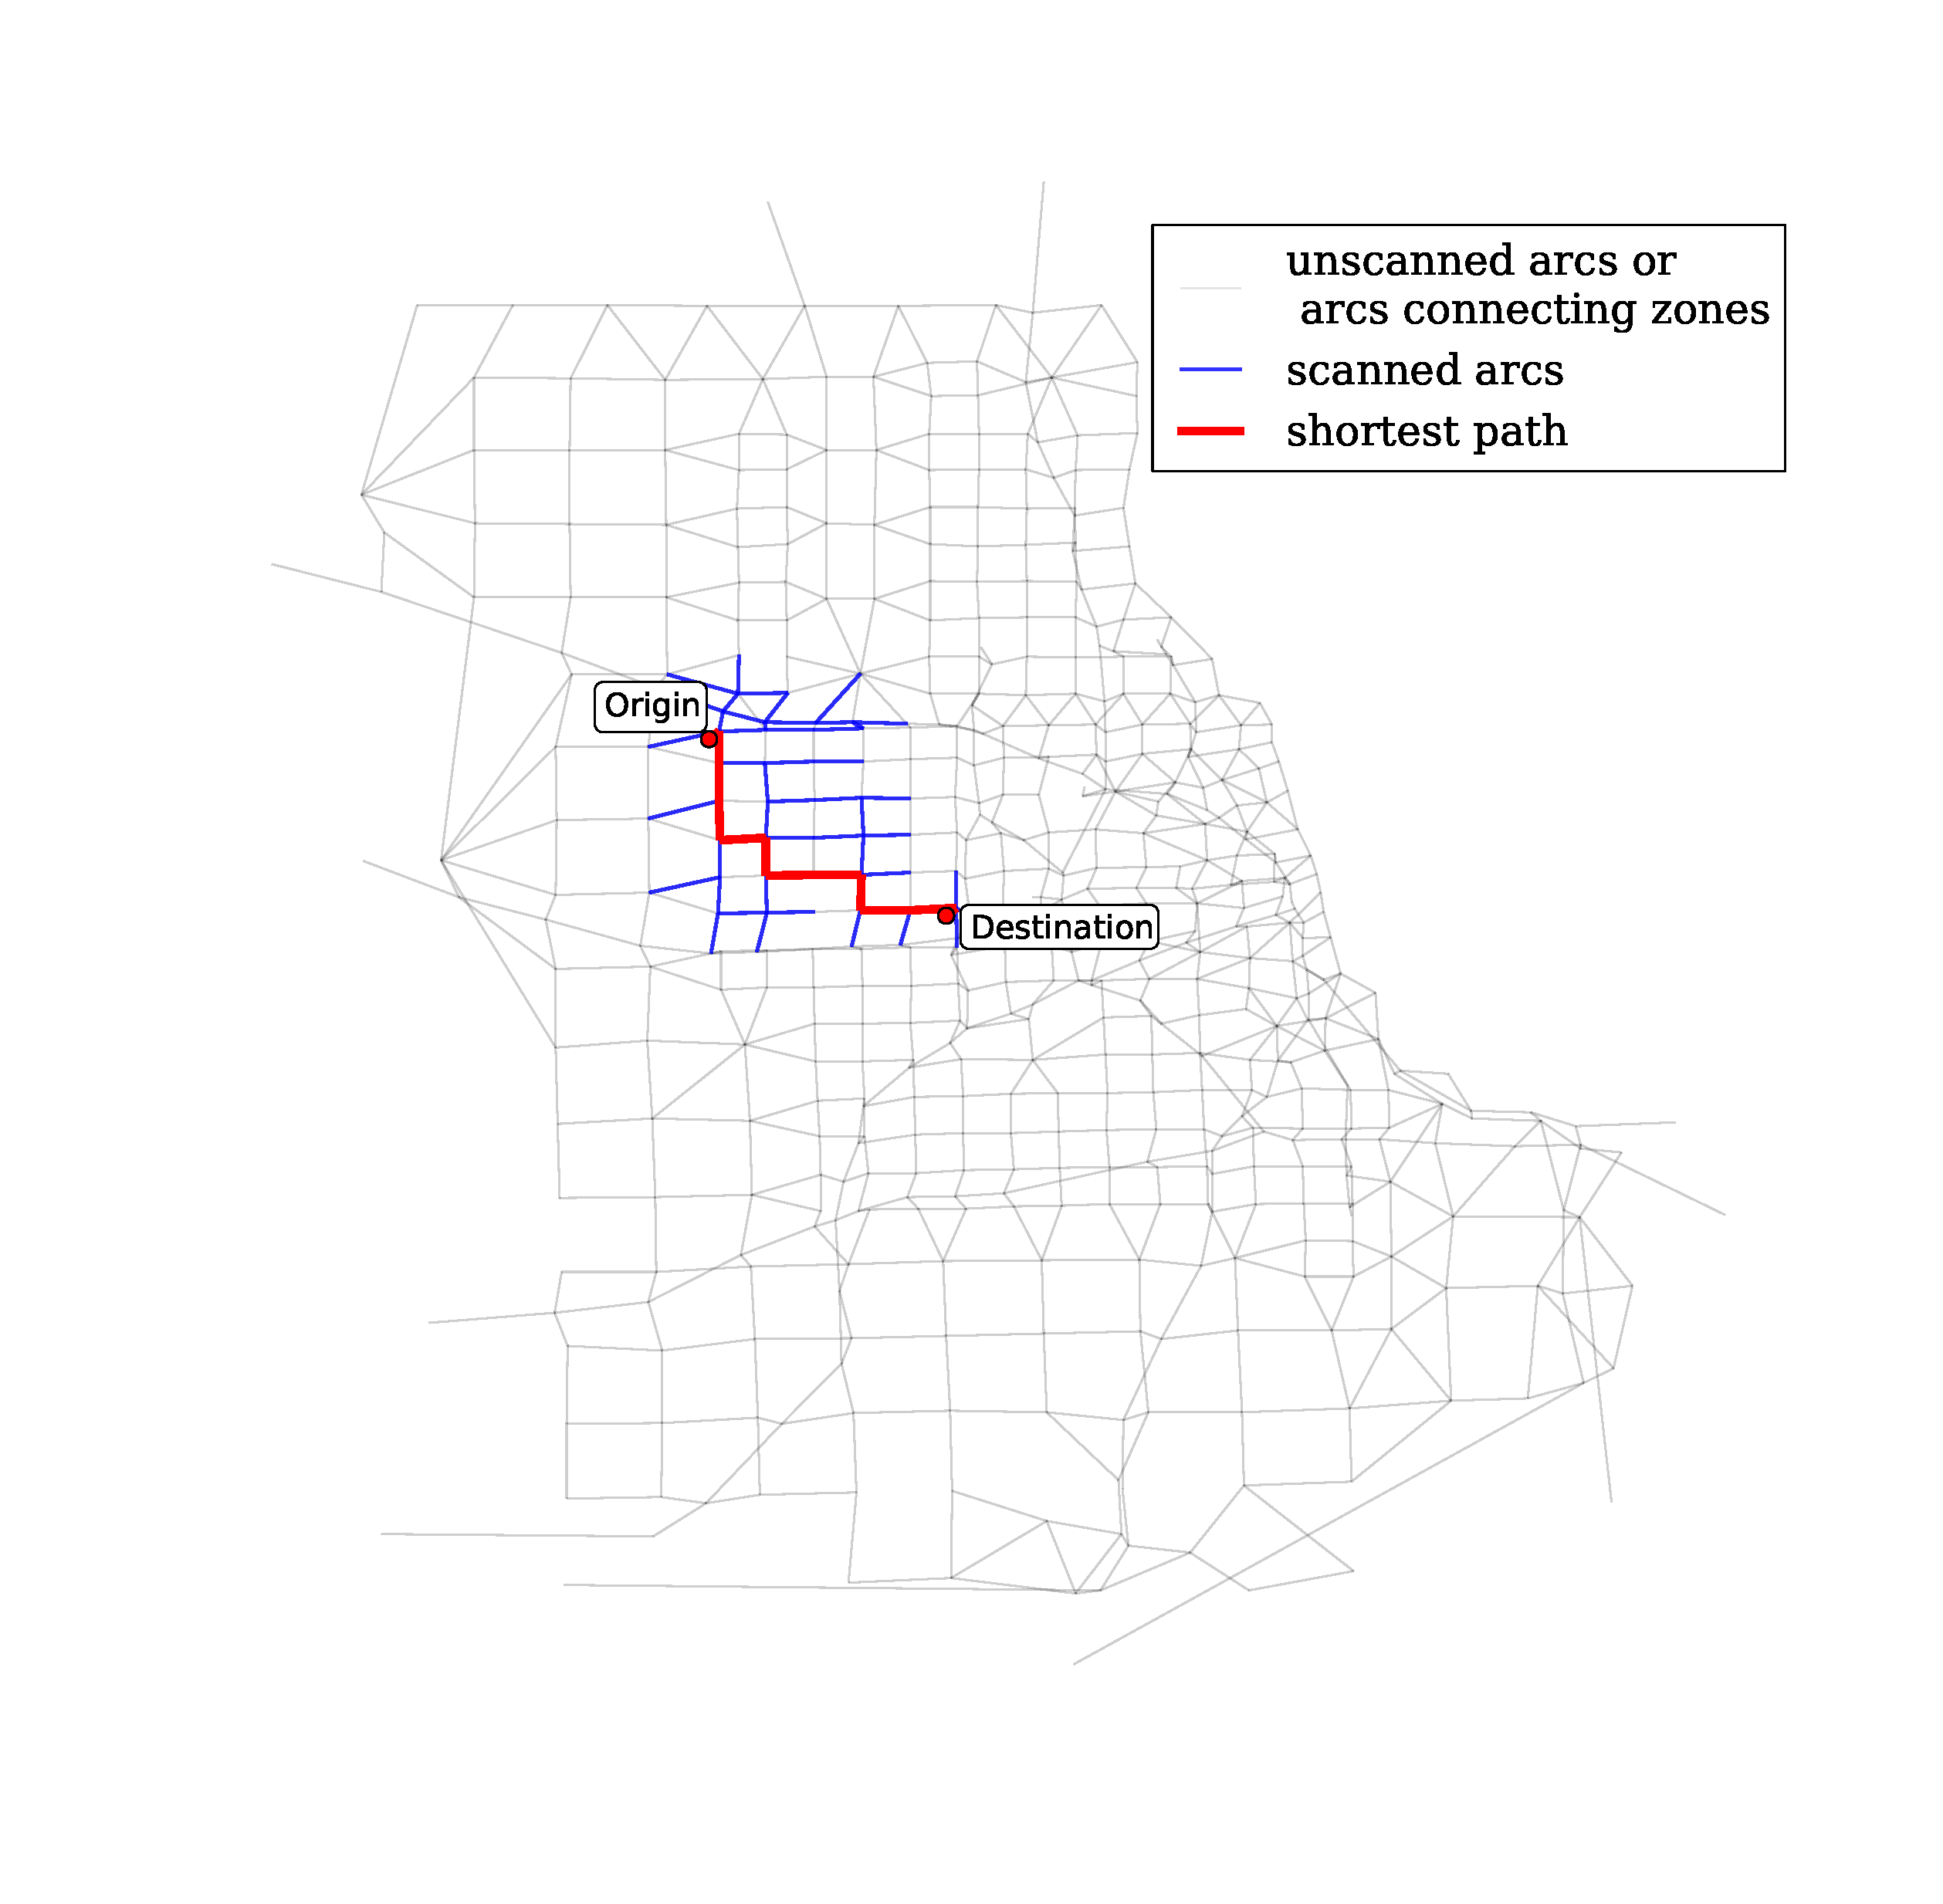
\includegraphics[width=\textwidth,trim=120px 120px 48px 0px,clip]{img/chicago_astar2}
        \caption{A* Search}
        \label{fig:chicago_astar2}
    \end{subfigure}%
    \begin{subfigure}{.5\textwidth}
        \centering
        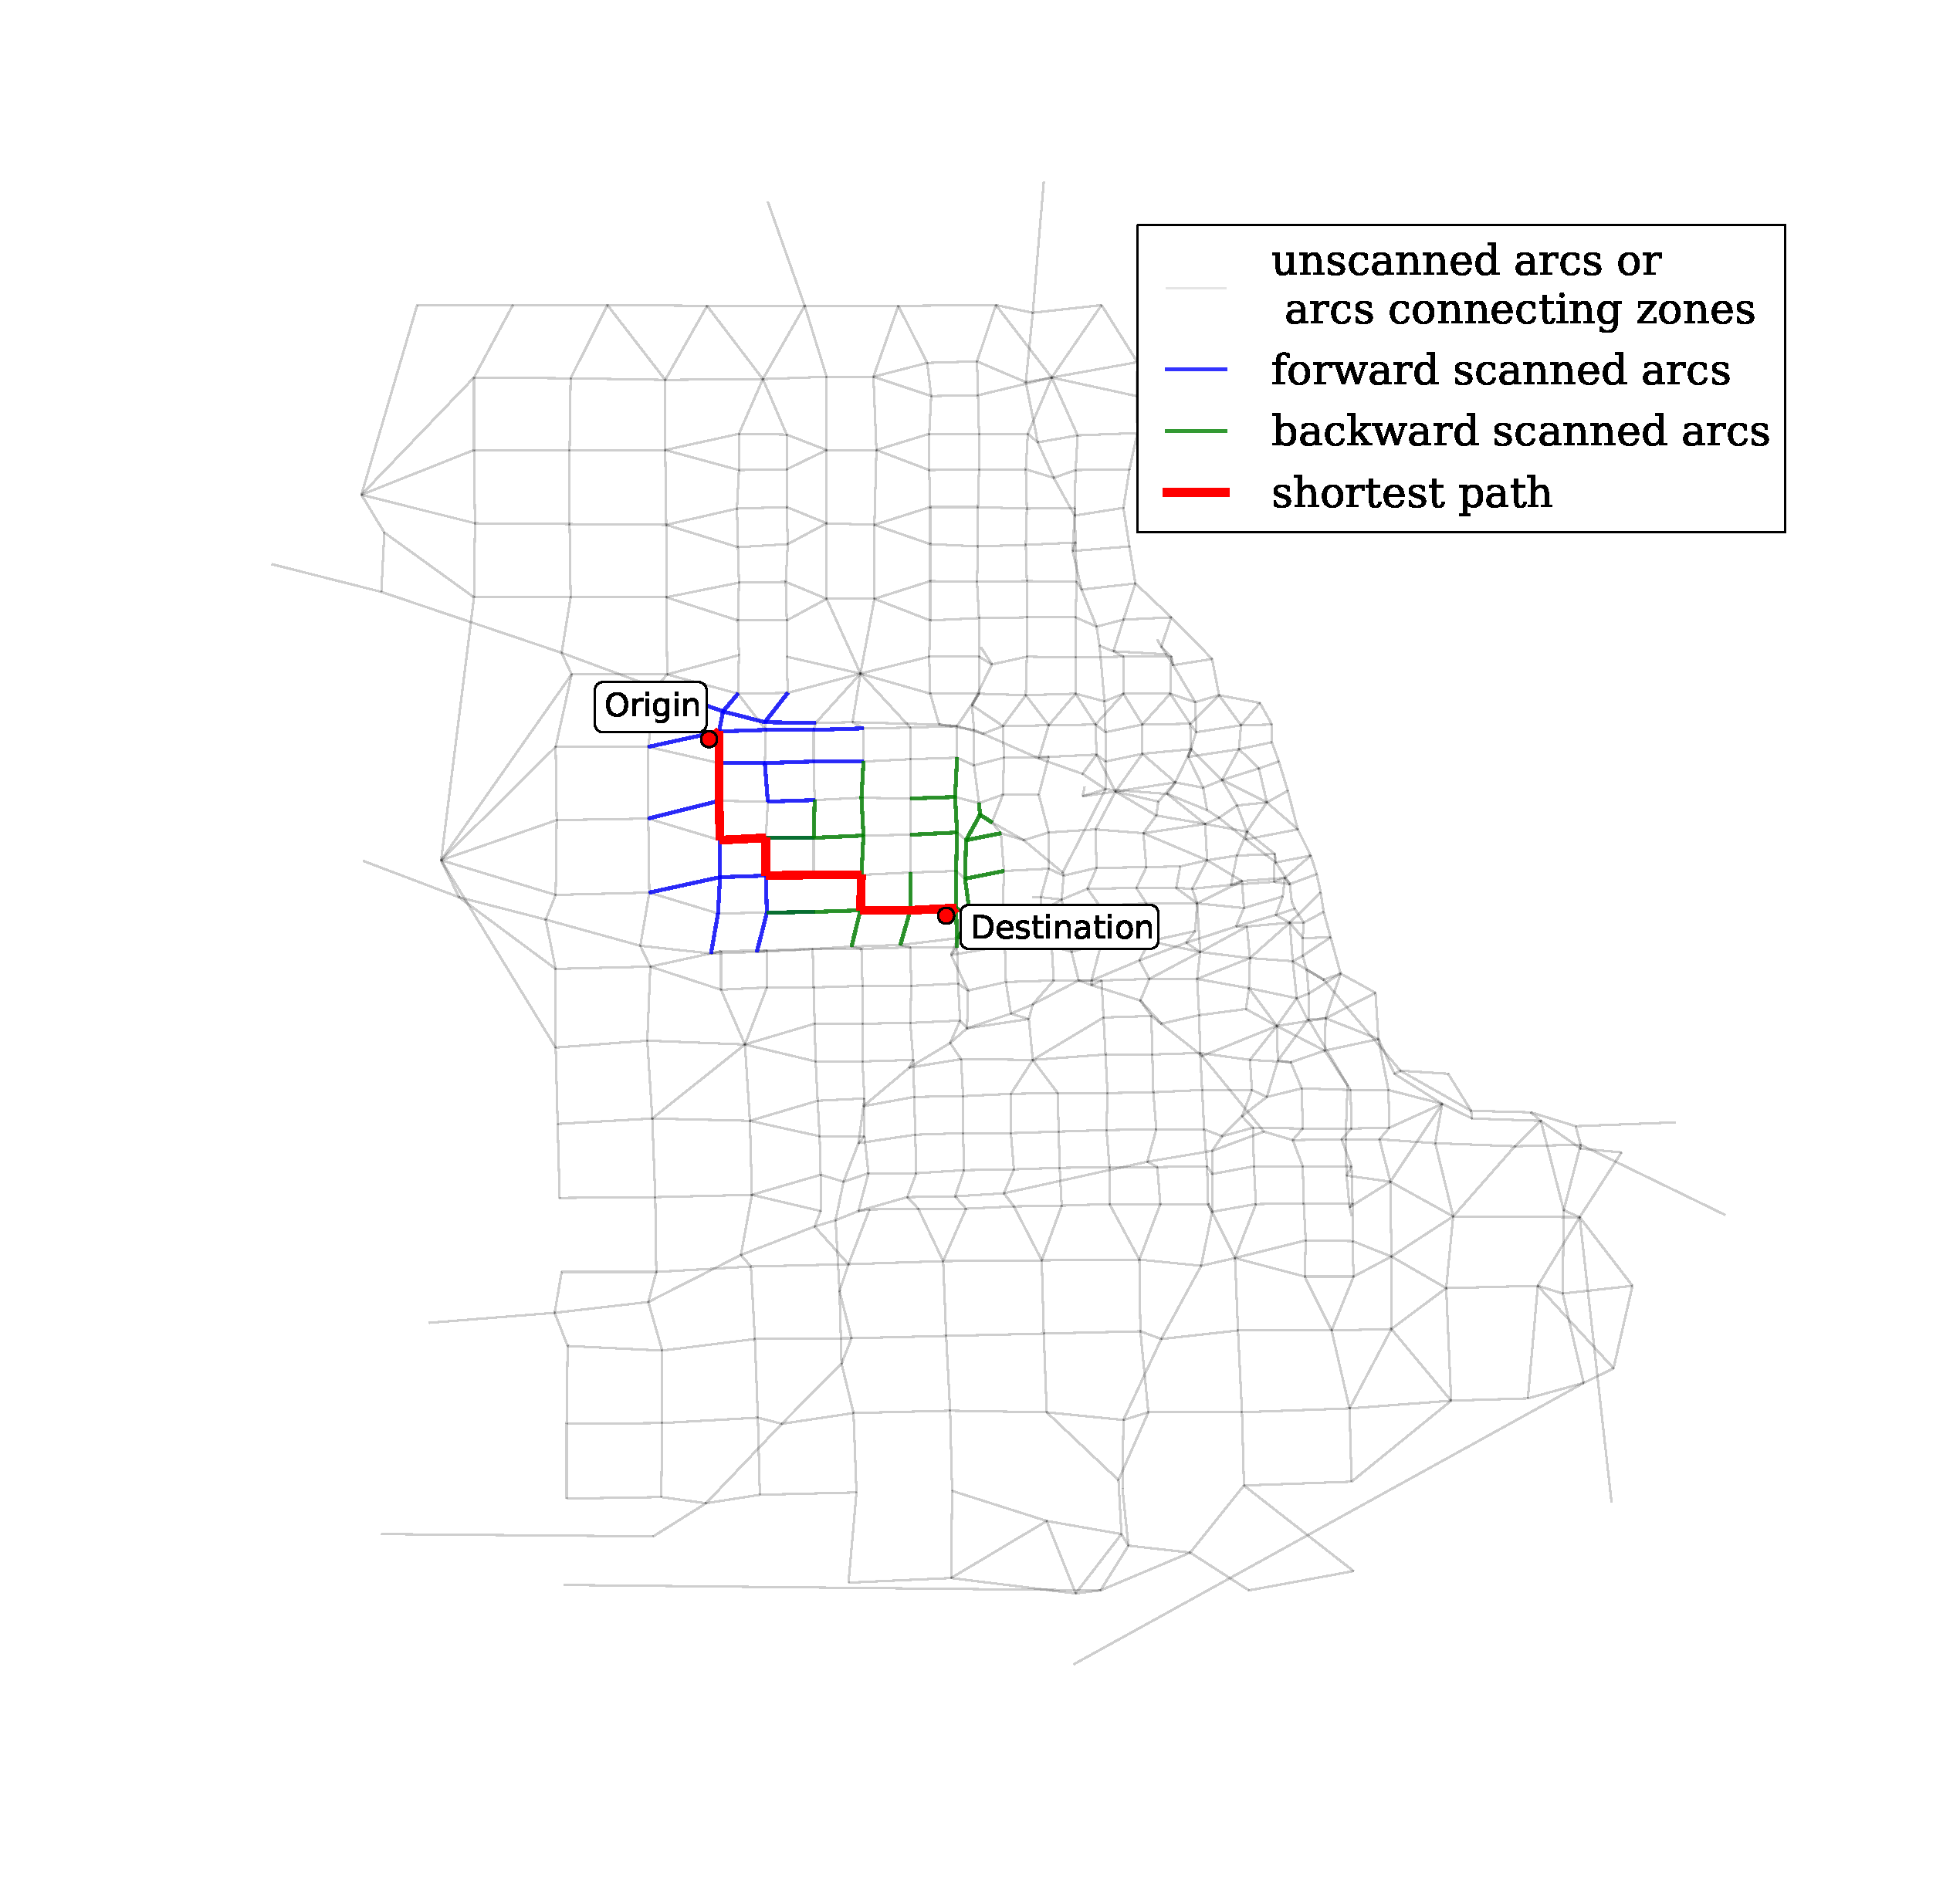
\includegraphics[width=\textwidth,trim=120px 120px 48px 0px,clip]{img/chicago_astar_bidirect2}
        \caption{Bidirectional A* Search}
        \label{fig:chicago_astar_bidirect2}
    \end{subfigure}
    \vspace{1em}
    \caption{Shortest path tree between two close nodes in the Chicago Sketch network}
    \label{fig:short_sptree}
\end{figure}

\section{A* search with landmarks}
A* search with landmarks algorithm is not implemented for this project.
This is due to its sophisticated graph dependent implementation,
where we need to either manually or dynamically decide the number of landmarks and their location placements.
And also there is a high chance of not being able to work efficiently,
as the algorithm is aimed at geographic node locations and Euclidean distances,
not travel times based on traffic flows.
Using zero-flow travel times may work but it was decided not to investigate this further.
Instead, we focus on strategies that avoid some of the shortest path computations altogether in the path equilibration algorithm.

